\documentclass[ xcolor = pdftex, dvipsnames, table ]{beamer}

\usetheme[compress]{Berlin}
\usecolortheme{whale}
\setlength{\parskip}{0.1in}
\usepackage{bm}
\usepackage{tikz}
\usepackage{dsfont}
\usepackage{graphicx}
\usepackage{changepage}
\usepackage{pgfgantt}
\usepackage{nicefrac}
\usepackage{scalerel}

%\title{Baysian Nonparametric Estimation of ODEs as Applied to the Stock Recruitment Relationship}
\title{Metamodeling for Bias Estimation of Biological Reference Points Under Two-Parameter SRRs}
\author{
Nick Grunloh
%\\$~$\\
%In collaboration with:\\
%Dr. E.J. Dick\\
%Dr. H. K.H. Lee
}
\date{14 March 2022}

\DeclareMathOperator*{\argmin}{\arg\!\min}
\DeclareMathOperator*{\argmax}{\arg\!\max}

%\newenvironment{changemargin}[2]{%
%\begin{list}{}{%
%\setlength{\topsep}{0pt}%
%\setlength{\leftmargin}{#1}%
%\setlength{\rightmargin}{#2}%
%\setlength{\listparindent}{\parindent}%
%\setlength{\itemindent}{\parindent}%
%\setlength{\parsep}{\parskip}%
%}%
%\item[]}{\end{list}}

%\AtBeginSection[]
%{
%    \begin{frame}
%        \frametitle{Table of Contents}
%        \tableofcontents[currentsection, currentsubsection]
%    \end{frame}
%}
%
%\AtBeginSubsection[]
%{
%    \begin{frame}
%        \frametitle{Table of Contents}
%        \tableofcontents[currentsection, currentsubsection]
%    \end{frame}
%}

%
\begin{document}

%
\begin{frame}
\titlepage
\vspace*{-3cm}
\begin{minipage}[h!]{0.49\textwidth}
\hspace*{-0.25cm}

\includegraphics[width=0.6\textwidth]{noaaText.png}
\end{minipage}
\begin{minipage}[h!]{0.49\textwidth}
\hspace*{2cm}

\includegraphics[width=0.55\textwidth]{slug.jpg}
\end{minipage}
\end{frame}

%
\begin{frame}{Outline}
    \tableofcontents
\end{frame}

%
\section{Introduction}
\subsection{}
\begin{frame}{Outline} 
    \tableofcontents[currentsection, currentsubsection]
\end{frame}

%
\begin{frame}{}
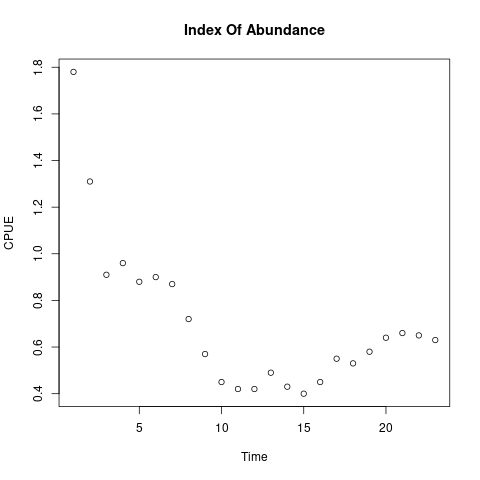
\includegraphics[width=0.49\textwidth]{../plots/hakeIndex.png}
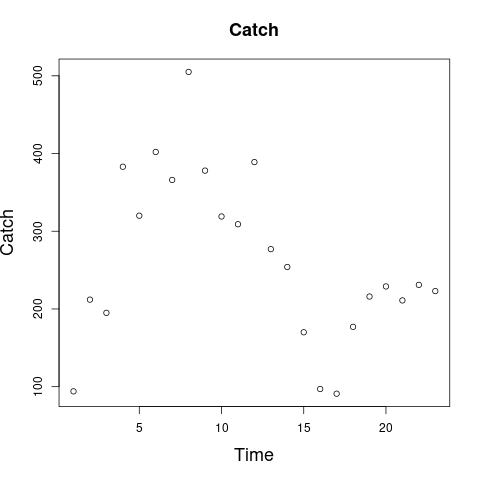
\includegraphics[width=0.49\textwidth]{../plots/hakeCatch.png}
\begin{align*}
I_t &= q B_t e^\epsilon ~~~ \epsilon\sim N(0, \sigma^2) \\
~\\
\frac{dB(t)}{dt} &= P(B(t);\bm{\theta}) - C(t)
\end{align*}
\end{frame}

%
\begin{frame}{Schaefer Model}
\begin{minipage}[h!]{0.44\textwidth}
\begin{align*}
        P_{\bm{\theta}}(B) &= rB\left(1-\frac{B}{K}\right)\\
	~\\
        \bm{\theta} &= (r, K)
	%\\~&~\\
        %\gamma &= 2 \Rightarrow \text{Schaefer Model}
\end{align*}
%\color{red}Maybe add one with parameters but without RPs
\end{minipage}
\begin{minipage}[h!]{0.54\textwidth}
%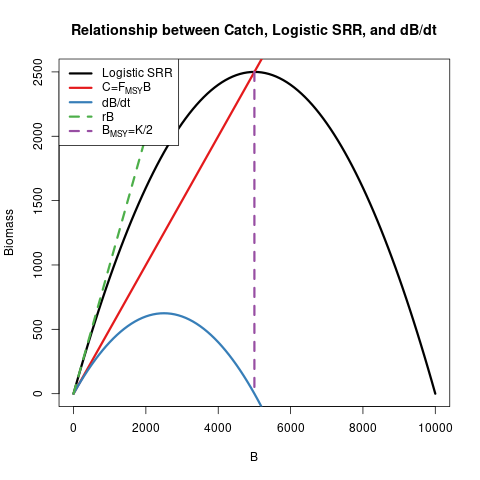
\includegraphics[width=\textwidth]{~../../.././nick/gpBias/srrSchaeffer.png}
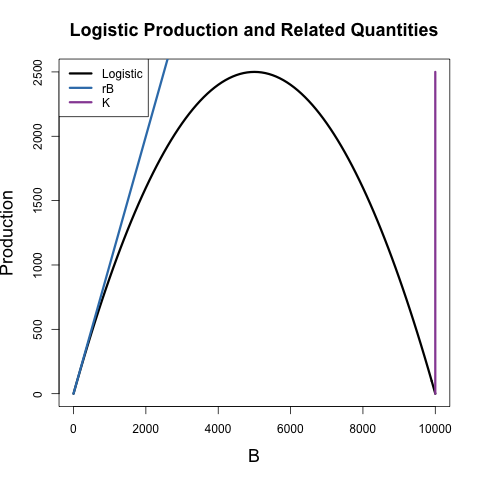
\includegraphics[width=1\textwidth]{../plots/srrSchaefferPar.png}
\end{minipage}
\end{frame}

%%
%\begin{frame}{}
%\begin{align}
%C(t) = F(t)B(t)
%\end{align}
%\color{red}
%something about catch\\
%and MSY derivation\\ 
%concept of equilibrium quantities\\
%Concept of MSY from my document\\
%Concept of RP from Punt
%\end{frame}

%
\begin{frame}{Schaefer Reference Points}
\begin{minipage}[h!]{0.44\textwidth}
\begin{align*}
        F^* &= \frac{r}{2}\\
	~\\
        \frac{B^*}{B_0}&= \frac{1}{2}\\
	~\\
        MSY &= \frac{rK}{4} 
\end{align*}
%\color{red}Maybe add one with only RPs
%\color{red}Add Mangle Citation
%{\color{red} Some words on RPs,  aybe some citations}
\end{minipage}
\begin{minipage}[h!]{0.54\textwidth}
%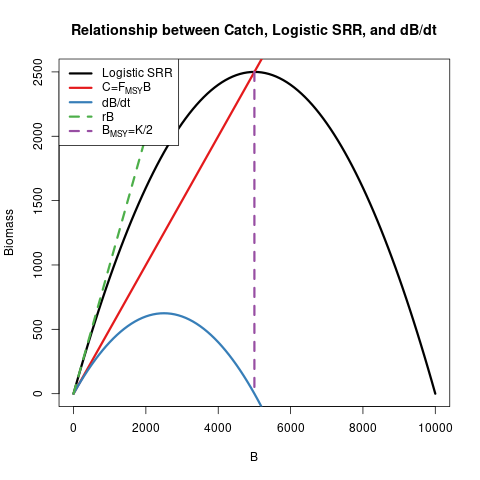
\includegraphics[width=\textwidth]{~../../.././nick/gpBias/srrSchaeffer.png}
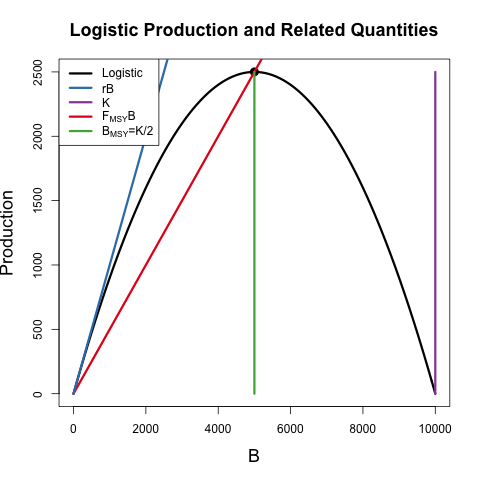
\includegraphics[width=1\textwidth]{../plots/srrSchaefferRPplus.png}
\end{minipage}
\end{frame}

%
\begin{frame}
\only<1>{
\hspace*{-0.5cm}
\begin{minipage}[h!]{0.59\textwidth}
Conceptually:
\begin{align*}
F^*\in\mathbb{R}^+ ~~~ \frac{B^*}{\bar B(0)}\in\left(0, 1\right)
\end{align*}
$~$\\
Mangel et al. 2013, CJFAS:
\begin{itemize}
	\item BH Model: $~ F^*\in\mathbb{R}^+ ~~~ \frac{B^*}{\bar B(0)}=\frac{1}{F^*/M+2}$
	\item Similar Constraint for Ricker and other 2 Parameter Curves
\end{itemize}
%\item A three-parameter relationship allows for independent estimation of these reference points
$~$\\
$~$\\
$~$\\
%Schaefer Model:
%\begin{align*}
%F^*\in\mathbb{R}^+ ~~~ \frac{B^*}{\bar B(0)}=\frac{1}{2}
%\end{align*}
\end{minipage}
\begin{minipage}[h!]{0.39\textwidth}
$~$\\
\hspace*{-0.5cm}
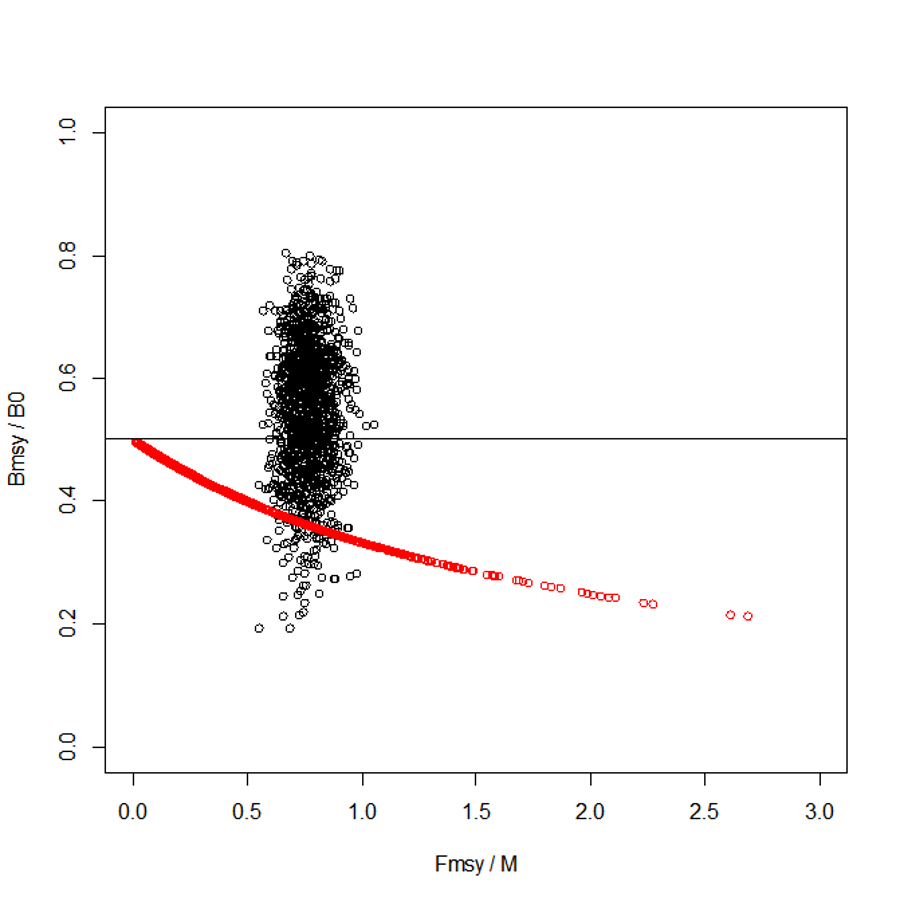
\includegraphics[width=1.4\textwidth]{cjasFig.png}
\end{minipage}
}
\only<2>{
\hspace*{-0.5cm}
\begin{minipage}[h!]{0.59\textwidth}
Conceptually:
\begin{align*}
F^*\in\mathbb{R}^+ ~~~ \frac{B^*}{\bar B(0)}\in\left(0, 1\right)
\end{align*}
$~$\\
Mangel et al. 2013, CJFAS:
\begin{itemize}
	\item BH Model: $~ F^*\in\mathbb{R}^+ ~~~ \frac{B^*}{\bar B(0)}=\frac{1}{F^*/M+2}$
	\item Similar Constraint for Ricker and other 2 Parameter Curves
\end{itemize}
%\item A three-parameter relationship allows for independent estimation of these reference points
$~$\\
Schaefer Model:
\begin{align*}
F^*\in\mathbb{R}^+ ~~~ \frac{B^*}{\bar B(0)}=\frac{1}{2}
\end{align*}
\end{minipage}
\begin{minipage}[h!]{0.39\textwidth}
$~$\\
\hspace*{-0.5cm}
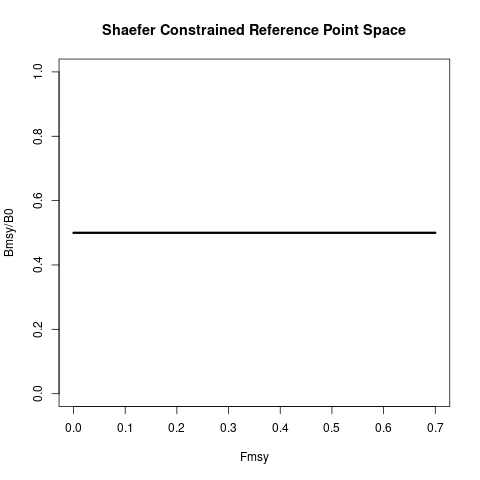
\includegraphics[width=1.4\textwidth]{shaeferConst.png}
\end{minipage}
}
\end{frame}

%
\section{Simulation}
\subsection{}
\begin{frame}{Outline}
    \tableofcontents[currentsection, currentsubsection]
\end{frame}

%
\begin{frame}{Pella-Tomlinson Production Model}
\begin{minipage}[h!]{0.54\textwidth}
\begin{align*}
        I(t) &\sim LN(qB(t), \sigma^2)\\
        \frac{dB(t)}{dt} &= P_{\bm{\theta}}(B(t)) - F(t)B(t)\\
	~&~\\
        P_{\bm{\theta}}(B) &= \frac{rB}{\gamma-1} \left(1-\frac{B}{K}\right)^{\gamma-1}\\
        \bm{\theta} &= (r, K, \gamma)\\
        ~&~\\
        \gamma &= 2 \Rightarrow \text{Schaefer Model}
\end{align*}
\end{minipage}
\begin{minipage}[h!]{0.44\textwidth}
%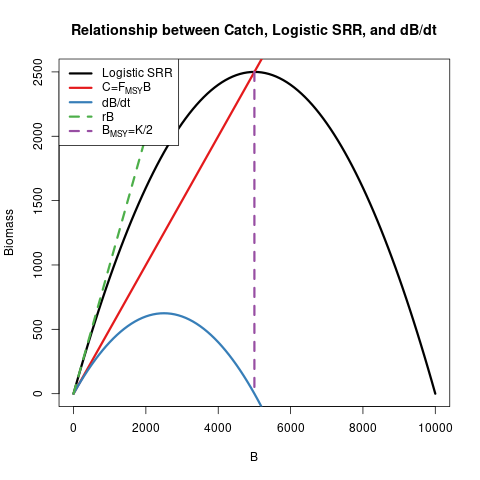
\includegraphics[width=\textwidth]{~../../.././nick/gpBias/srrSchaeffer.png}
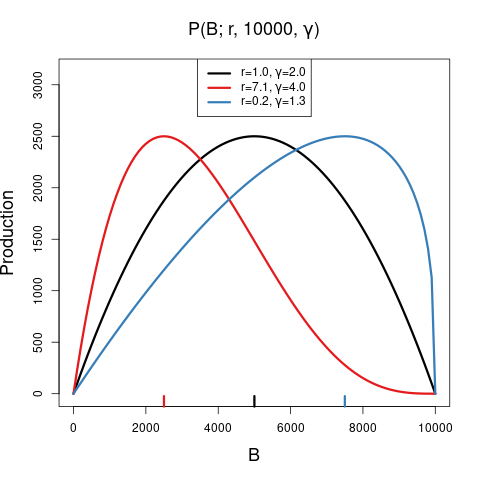
\includegraphics[width=1.15\textwidth]{../plots/srr1.1.png}
\end{minipage}
\end{frame}

%%
%\begin{frame}{Catch}
%\only<1>{
%\vspace*{-0.1cm}
%\begin{center}
%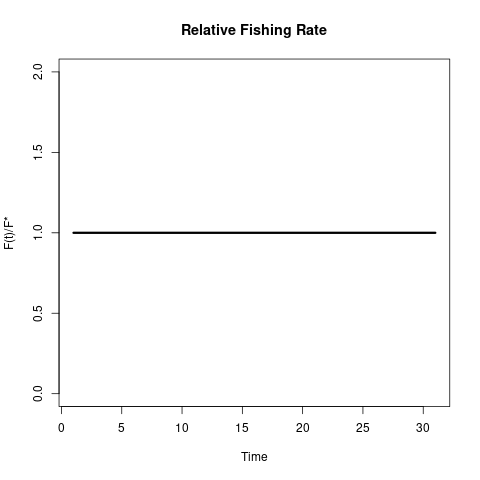
\includegraphics[width=0.32\textwidth]{../../.././nick/gpBias/rfFlatNoQX2Z0.6.png}
%\hspace*{1cm}
%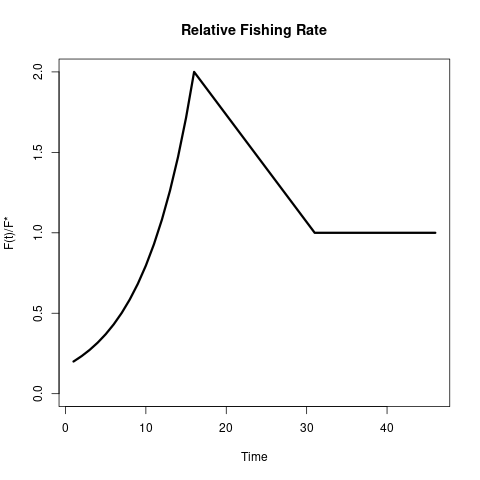
\includegraphics[width=0.32\textwidth]{../../.././nick/gpBias/rfExpT45X2Z0.6.png}
%%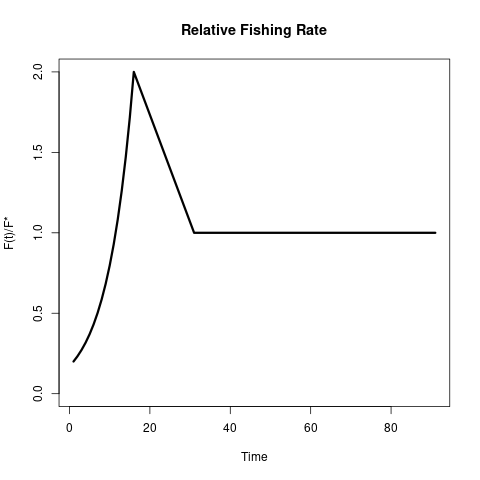
\includegraphics[width=0.32\textwidth]{../../.././nick/gpBias/rfExpT90X2Z0.6.png}
%\end{center}
%\begin{align*}
%C(t) &= F(t)B(t)\\
%&= F^*\left(\frac{F(t)}{F^*}\right)B(t)\\
%\end{align*}
%}
%\only<2>{
%\vspace*{-0.1cm}
%\begin{center}
%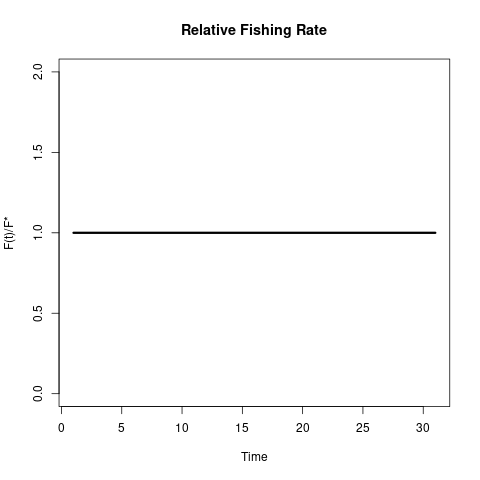
\includegraphics[width=0.32\textwidth]{../../.././nick/gpBias/rfFlatNoQX2Z0.6.png}
%\hspace*{1cm}
%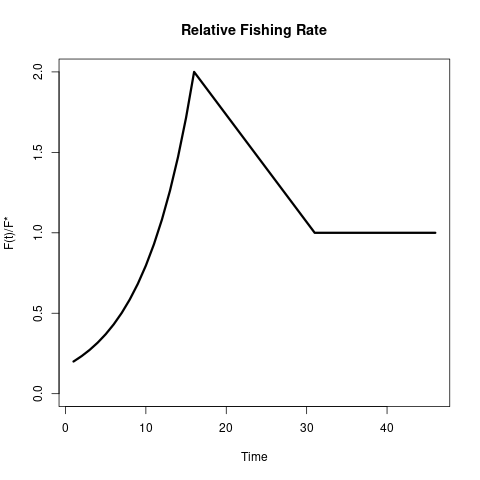
\includegraphics[width=0.32\textwidth]{../../.././nick/gpBias/rfExpT45X2Z0.6.png}\\
%%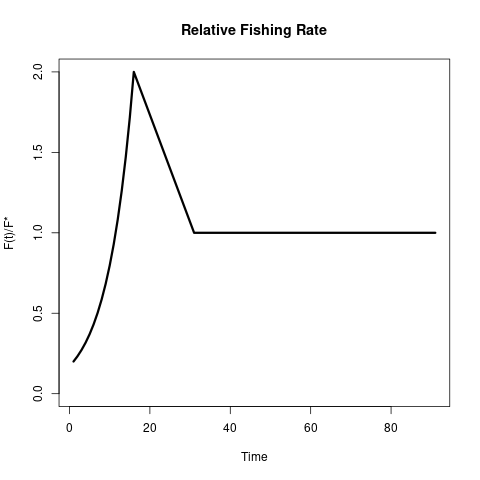
\includegraphics[width=0.32\textwidth]{../../.././nick/gpBias/rfExpT90X2Z0.6.png}\\
%\vspace*{-0.1cm}
%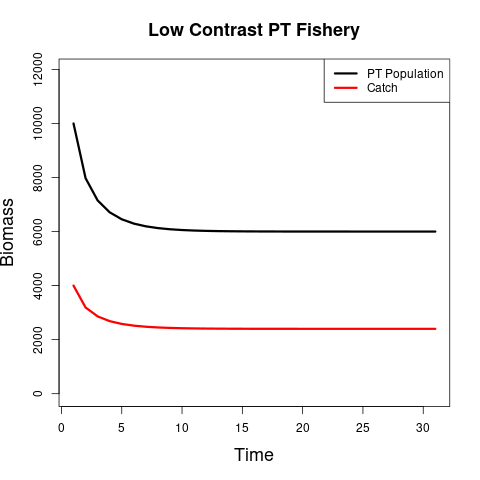
\includegraphics[width=0.32\textwidth]{../../.././nick/gpBias/bioCatchFlatNoQX2Z0.6.png}
%\hspace*{1cm}
%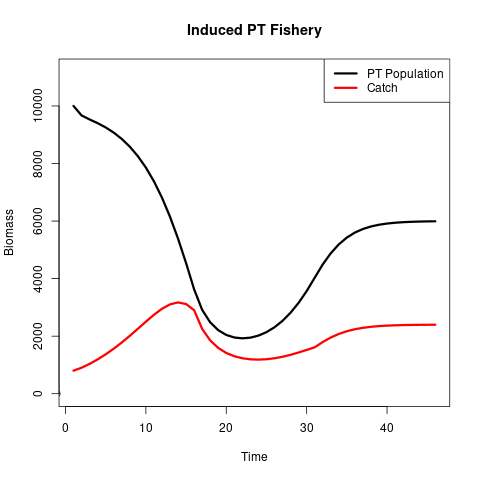
\includegraphics[width=0.32\textwidth]{../../.././nick/gpBias/bioCatchExpT45X2Z0.6.png}
%%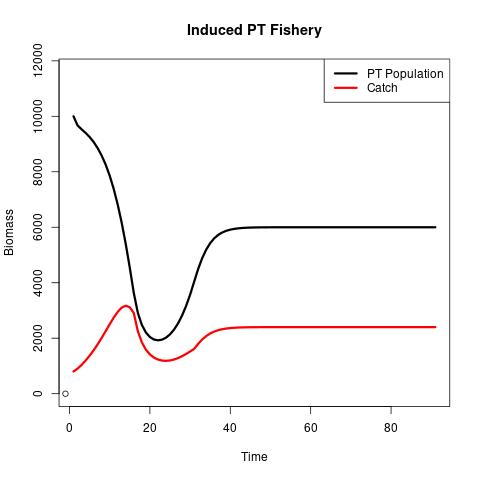
\includegraphics[width=0.32\textwidth]{../../.././nick/gpBias/bioCatchExpT90X2Z0.6.png}
%\end{center}
%}
%\end{frame}

%
\begin{frame}{Catch}
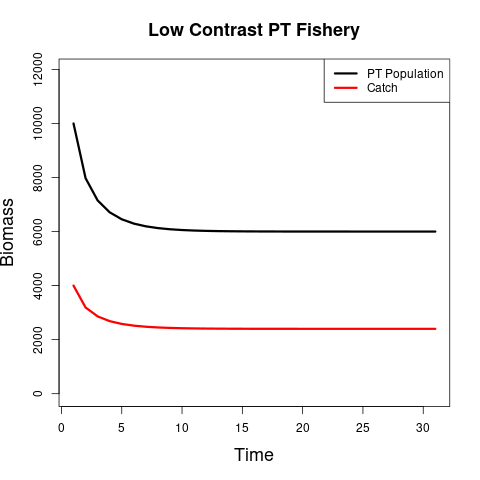
\includegraphics[width=0.49\textwidth]{../../.././nick/gpBias/bioCatchFlatNoQX2Z0.6.png}
%\hspace*{1cm}
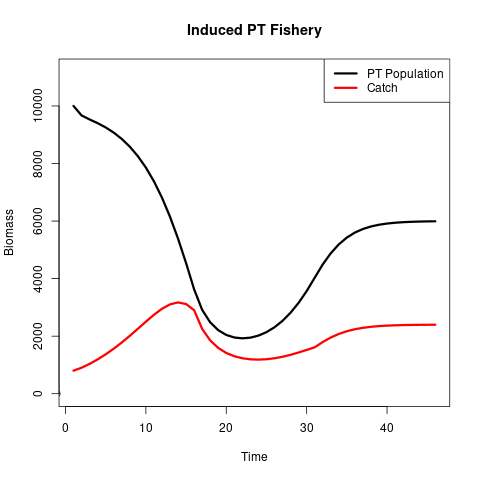
\includegraphics[width=0.49\textwidth]{../../.././nick/gpBias/bioCatchExpT45X2Z0.6.png}
\end{frame}

%
\begin{frame}
\only<1>{
\vspace{-0.5cm}
\begin{align*}
\hspace*{-0.5cm}
\bm{\theta}=\left[r = F^*\left( \frac{1-\frac{B^*}{\bar B(0)}}{\frac{B^*}{\bar B(0)}} \right) \left(1-\frac{B^*}{\bar B(0)}\right)^{\left( \frac{\frac{B^*}{\bar B(0)}-1}{\frac{B^*}{\bar B(0)}} \right)},~K = 10000, ~\gamma = \frac{1}{\frac{B^*}{\bar B(0)}}\right]
\end{align*}
$~$\\
\vspace*{-0.65cm}
\hspace*{1.72cm}
\begin{tikzpicture}
%\begin{center}
\node (img) at (0,0) 
	{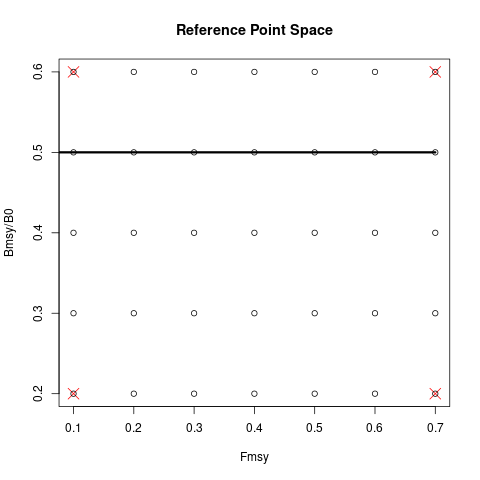
\includegraphics[height=0.8\textheight]{shaeferDat.png}};
%\node (tol) at (-4,1.5) 
%	{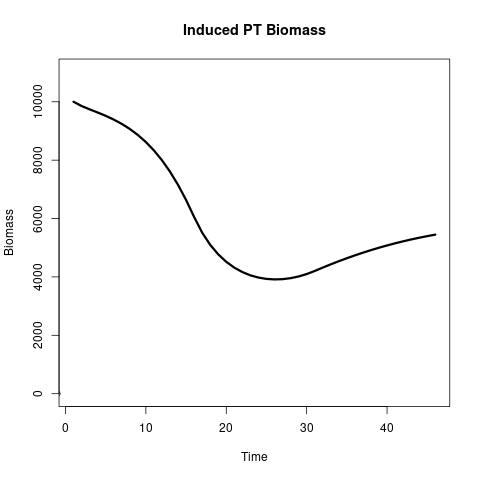
\includegraphics[height=0.25\textheight]{../../.././nick/gpBias/bioExpT45X0.5Z0.6.png}};
%\node (tor) at (4,1.5) 
%	{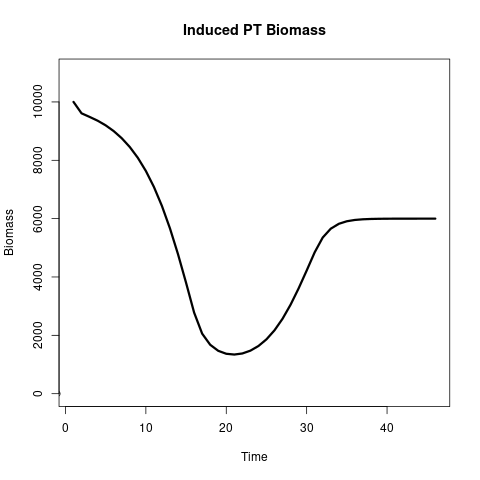
\includegraphics[height=0.25\textheight]{../../.././nick/gpBias/bioExpT45X3.5Z0.6.png}};
%\node (bor) at (4,-1.5) 
%	{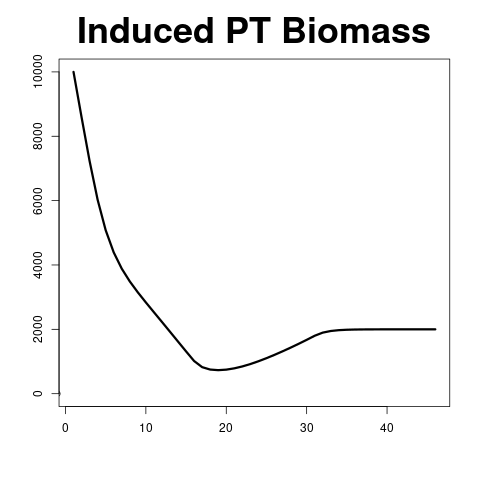
\includegraphics[height=0.25\textheight]{../../.././nick/gpBias/bioExpT45X3.5Z0.2.png}};
%\node (bol) at (-4,-1.5) 
%	{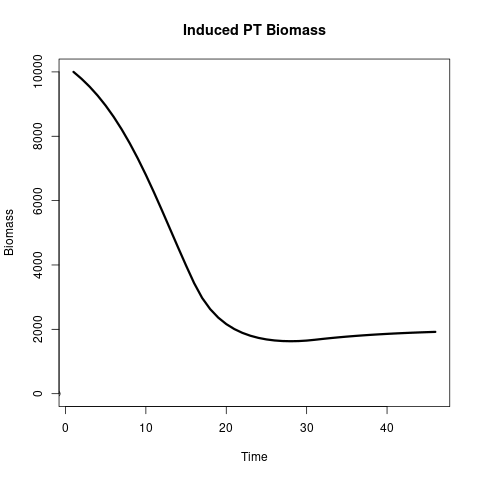
\includegraphics[height=0.25\textheight]{../../.././nick/gpBias/bioExpT45X0.5Z0.2.png}};
\end{tikzpicture}
}
\only<2>{
\vspace{-0.5cm}
\begin{align*}
\hspace*{-0.5cm}
\bm{\theta}=\left[r = F^*\left( \frac{1-\frac{B^*}{\bar B(0)}}{\frac{B^*}{\bar B(0)}} \right) \left(1-\frac{B^*}{\bar B(0)}\right)^{\left( \frac{\frac{B^*}{\bar B(0)}-1}{\frac{B^*}{\bar B(0)}} \right)},~K = 10000, ~\gamma = \frac{1}{\frac{B^*}{\bar B(0)}}\right]
\end{align*}
$~$\\
\vspace*{-0.65cm}
\begin{tikzpicture}
%\begin{center}
\node (img) at (0,0) 
	{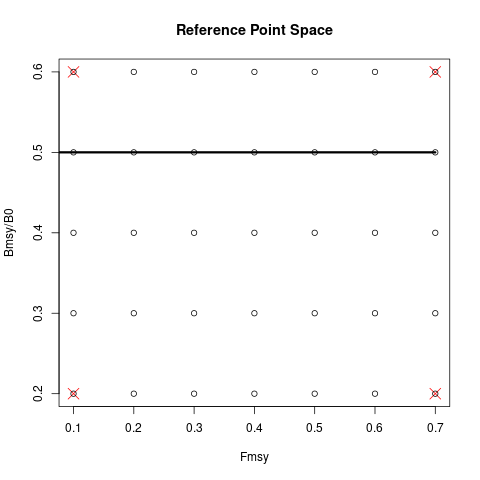
\includegraphics[height=0.8\textheight]{shaeferDat.png}};
\node (tol) at (-4,1.5) 
	{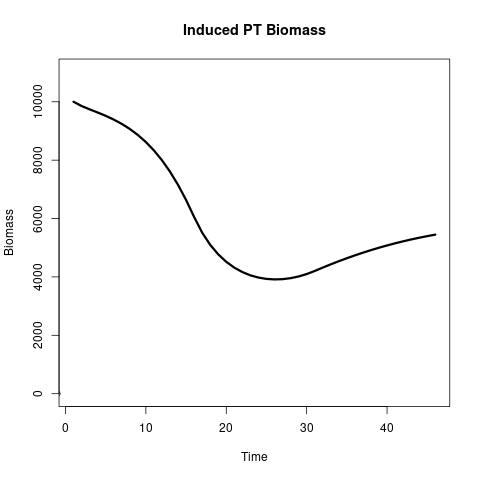
\includegraphics[height=0.25\textheight]{../../.././nick/gpBias/bioExpT45X0.5Z0.6.png}};
\node (tor) at (4,1.5) 
	{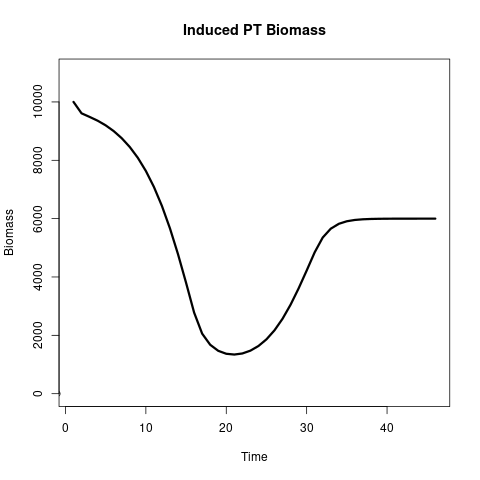
\includegraphics[height=0.25\textheight]{../../.././nick/gpBias/bioExpT45X3.5Z0.6.png}};
\node (bor) at (4,-1.5) 
	{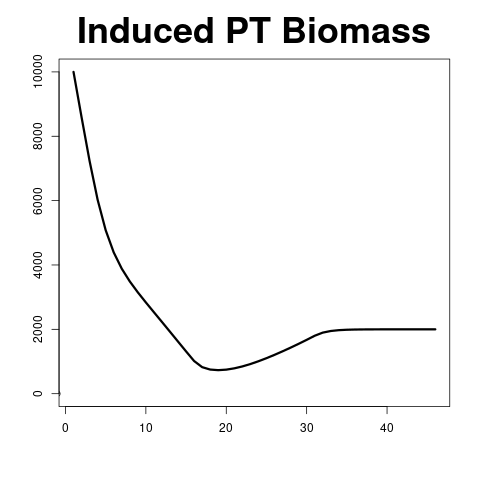
\includegraphics[height=0.25\textheight]{../../.././nick/gpBias/bioExpT45X3.5Z0.2.png}};
\node (bol) at (-4,-1.5) 
	{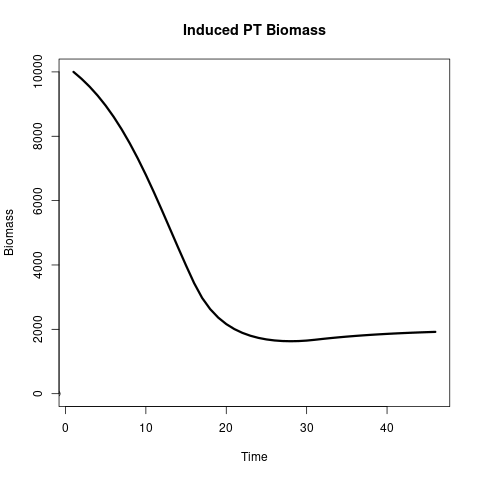
\includegraphics[height=0.25\textheight]{../../.././nick/gpBias/bioExpT45X0.5Z0.2.png}};
\end{tikzpicture}
}
\end{frame}

%
\begin{frame}{Metamodel}

\begin{equation*}
\underbrace{\left(F^*, \frac{B^*}{\bar B(0)}\right)}_{\text{PT Truth}} {\text{GP}\atop{\mapsto\atop~}} \underbrace{\left(\hat F^*, \frac{\hat B^*}{\bar B(0)}\right)}_{\text{Shaefer Estimate}}
\end{equation*}

\begin{itemize}
\item GP interpolates over degrees of RP model misspecification.
\item Propogation of estimate uncertainty smooths bias estimation.
\item Explicitely highlights trade-offs induced in RPs.
\end{itemize}
%
\end{frame}

%
\section{Results}
\subsection{Low Contrast}
\begin{frame}{Outline}
%
$~$\\
\tableofcontents[currentsection, currentsubsection]
%
\tikz[remember picture,overlay]
 \node at (8,3.5) %([xshift=-2.5cm,yshift=-1.5cm]current page.north east) 
  {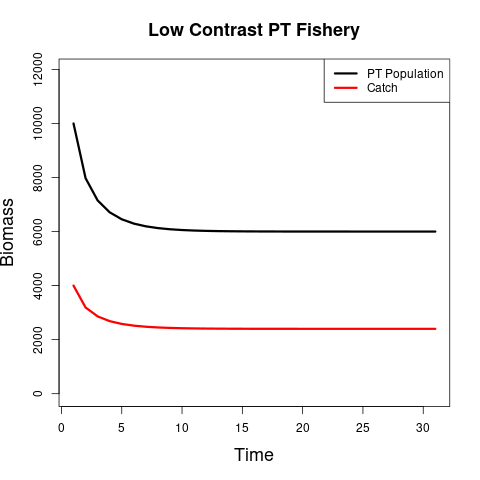
\includegraphics[width=0.5\textwidth]{../../.././nick/gpBias/bioCatchFlatNoQX2Z0.6.png}};
%
\end{frame}

%
\begin{frame}
%$~$\\
%\vspace*{-0.5cm}
%\hspace*{-1.54cm}
%\begin{minipage}[h!]{0.325\textwidth}
%\hspace*{0.25cm}
%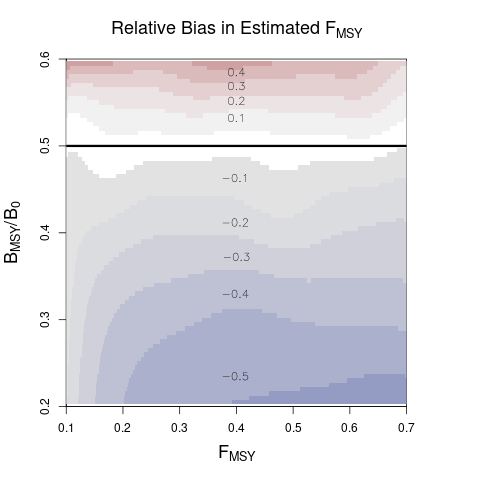
\includegraphics[width=1.2\textwidth]{../../.././nick/gpBias/fMSYRelBiasPellaFlatNoQ.png}
%\end{minipage}
%\begin{minipage}[h!]{0.325\textwidth}
%\hspace*{1cm}
%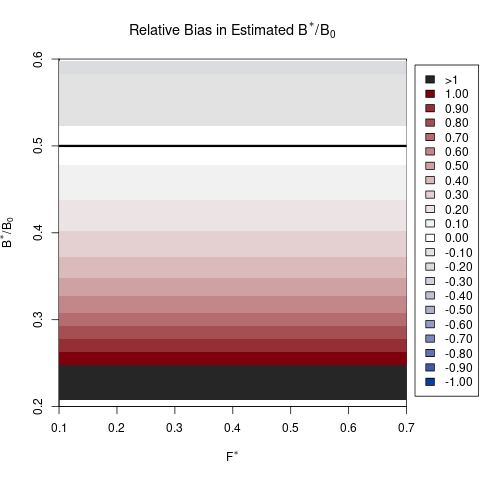
\includegraphics[width=1.2\textwidth]{../../.././nick/gpBias/zetaRelBiasPellaFlatNoQ.png}
%\end{minipage}
%\begin{minipage}[h!]{0.325\textwidth}
%\hspace*{1.6cm}
\begin{center}
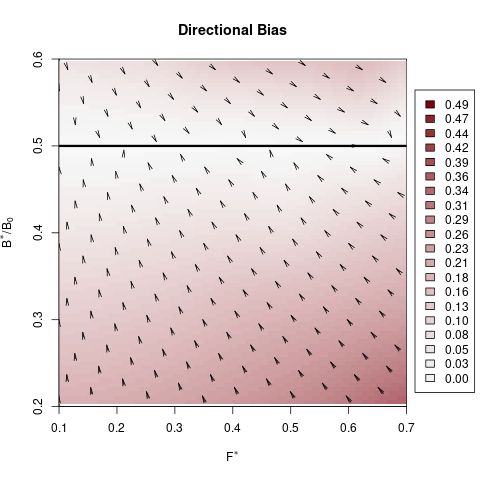
\includegraphics[height=\textheight]{../../.././nick/gpBias/directionalBiasPellaFlatNoQ.png}
\end{center}
%\end{minipage}
\end{frame}

%
\begin{frame}{Components of Bias}
$~$\\
\vspace*{-0.5cm}
\hspace*{-1cm}
\begin{minipage}[h!]{0.49\textwidth}
\hspace*{0.25cm}
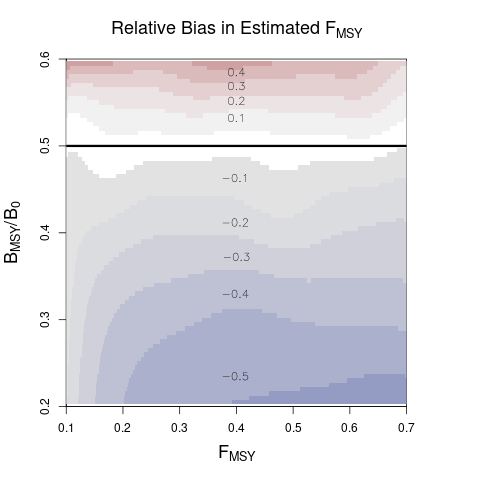
\includegraphics[width=1.1\textwidth]{../../.././nick/gpBias/fMSYRelBiasPellaFlatNoQ.png}
\end{minipage}
\begin{minipage}[h!]{0.49\textwidth}
\hspace*{1cm}
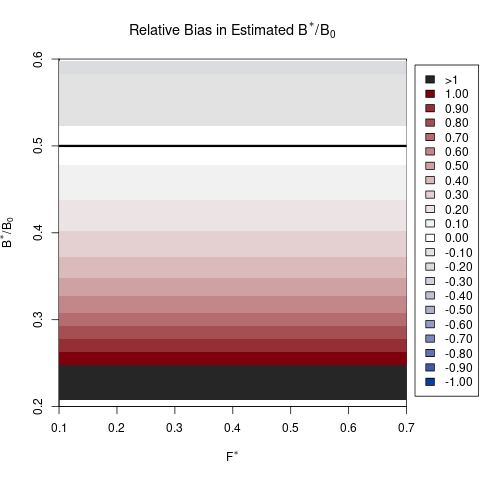
\includegraphics[width=1.1\textwidth]{../../.././nick/gpBias/zetaRelBiasPellaFlatNoQ.png}
\end{minipage}
%\begin{minipage}[h!]{0.325\textwidth}
%\hspace*{1.6cm}
%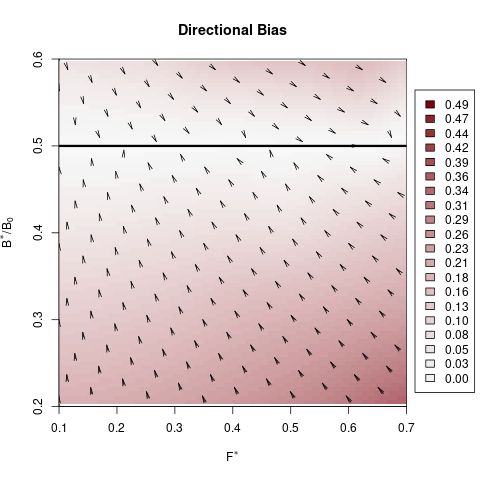
\includegraphics[width=1.2\textwidth]{../../.././nick/gpBias/directionalBiasPellaFlatNoQ.png}
%\end{minipage}
\end{frame}

%
\begin{frame}%{Understanding $F^*$ Bias Mechanisms}
%$~$\\
%\vspace*{-0.5cm}
\begin{minipage}[h!]{0.325\textwidth}
\hspace*{-1cm}
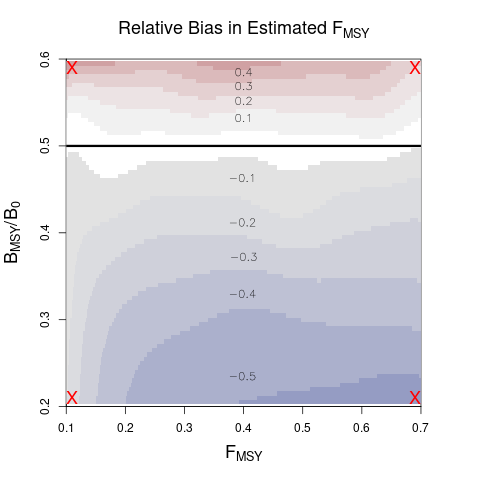
\includegraphics[width=1.25\textwidth]{../../.././nick/gpBias/fMSYXRelBiasPellaFlatNoQ.png}
\end{minipage}
\begin{minipage}[h!]{0.325\textwidth}
%\hspace*{1cm}
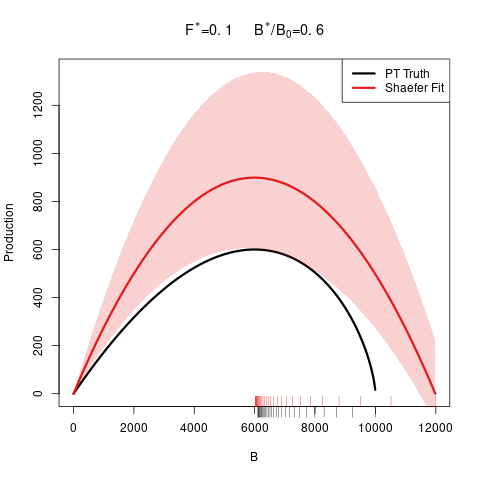
\includegraphics[width=1.1\textwidth]{../../.././nick/gpBias/curveCompareFlatNoQX0.5Z0.6.png}\\
%\vspace*{1.5cm}
%\hspace*{1cm}
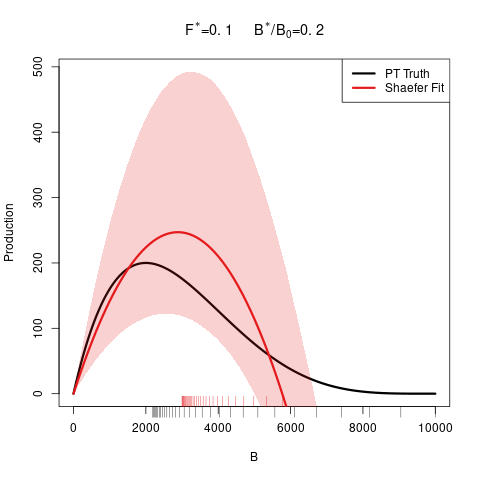
\includegraphics[width=1.1\textwidth]{../../.././nick/gpBias/curveCompareFlatNoQX0.5Z0.2.png}
\end{minipage}
\begin{minipage}[h!]{0.325\textwidth}
\hspace*{0.25cm}
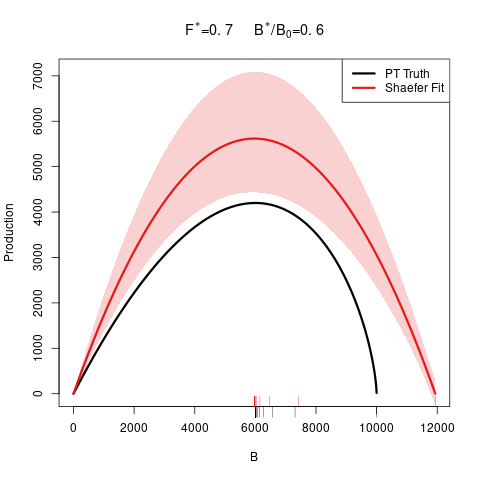
\includegraphics[width=1.1\textwidth]{../../.././nick/gpBias/curveCompareFlatNoQX3.5Z0.6.png}\\
%\vspace*{-0.5cm}
\hspace*{0.25cm}
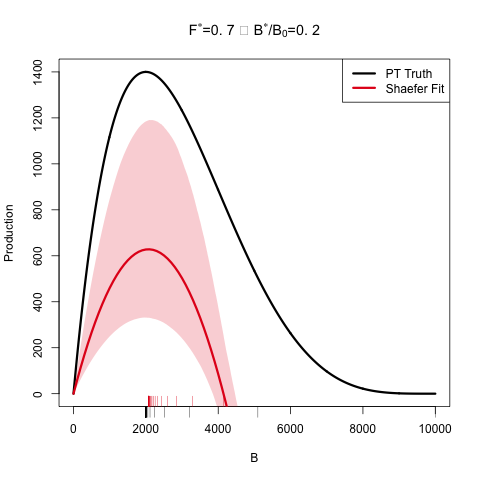
\includegraphics[width=1.1\textwidth]{../../.././nick/gpBias/curveCompareFlatNoQX3.5Z0.2.png}
\end{minipage}
%{\color{red} add $F^*$ Story words}
\end{frame}

%
\begin{frame}%{Split $\frac{B^*}{B_0}$}
%\begin{equation*}
%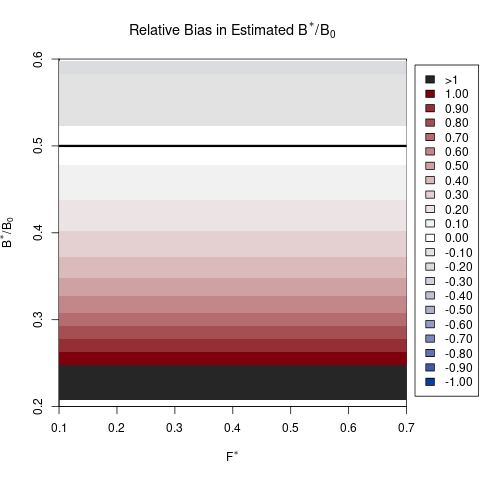
\includegraphics[width=0.33\textwidth]{../../.././nick/gpBias/zetaRelBiasPellaFlatNoQ.png}
%=
%\stretchleftright[500]{.}{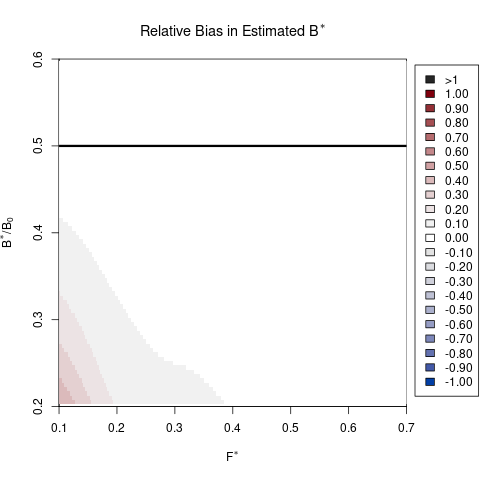
\includegraphics[width=0.4\textwidth]{../../.././nick/gpBias/bMSYRelBiasPellaFlatNoQ.png}}{/}
%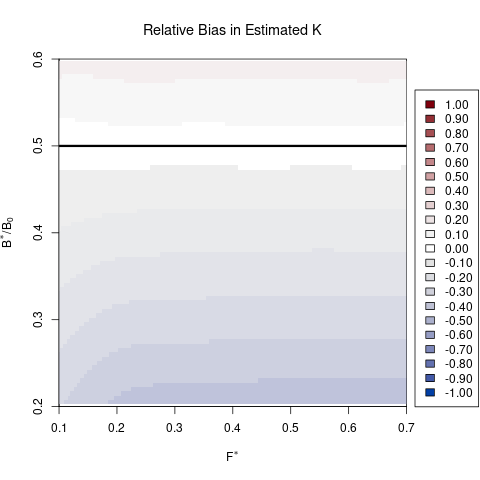
\includegraphics[width=0.4\textwidth]{../../.././nick/gpBias/kRelBiasPellaFlatNoQ.png}
%%\left.
%%\vspace*{1cm}
%%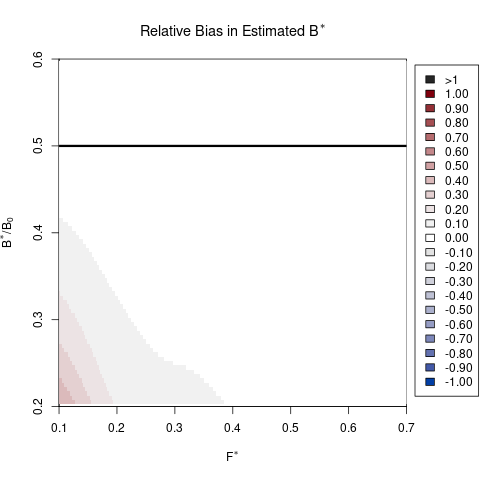
\includegraphics[width=0.4\textwidth]{../../.././nick/gpBias/bMSYRelBiasPellaFlatNoQ.png}
%%\middle/
%%\vspace*{-1cm}
%%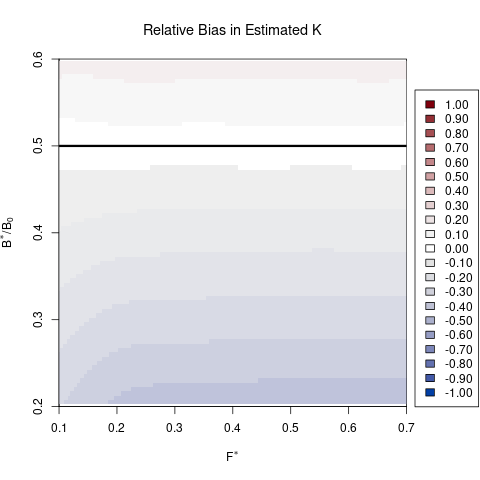
\includegraphics[width=0.4\textwidth]{../../.././nick/gpBias/kRelBiasPellaFlatNoQ.png}\right.
%\end{equation*}
\begin{minipage}[h!]{0.49\textwidth}
%\hspace*{-0.75cm}
$~$\\\\
\includegraphics[height=0.55\textheight]{../../.././nick/gpBias/zetaRelBiasPellaFlatNoQ.png}
\end{minipage}
\begin{minipage}[h!]{0.49\textwidth}
\hspace*{-0.5cm}
%\vspace*{1.5cm}
%\includegraphics[height=0.55\textheight]{../../.././nick/gpBias/bMSYRelBiasPellaFlatNoQ.png}\\
\hspace*{-0.5cm}
%\vspace*{1cm}
%\includegraphics[height=0.55\textheight]{../../.././nick/gpBias/kRelBiasPellaFlatNoQ.png}
\begin{tikzpicture}
\node (img) at (0,0)
        {\includegraphics[height=0.55\textheight]{../../.././nick/gpBias/bMSYRelBiasPellaFlatNoQ.png}};
\node (img) at (0,-3.75)
        {\includegraphics[height=0.55\textheight]{../../.././nick/gpBias/kRelBiasPellaFlatNoQ.png}};
\draw [latex-latex](-4,-1.75) -- (-2.5,0);
\draw [latex-latex](-4,-2.25) -- (-2.5,-4);
\end{tikzpicture}
\end{minipage}
\end{frame}



%
\subsection{High Contrast}
\begin{frame}{Outline}
%
$~$\\
\tableofcontents[currentsection, currentsubsection]
%
\tikz[remember picture,overlay]
 \node at (8,3.5) %([xshift=-2.5cm,yshift=-1.5cm]current page.north east) 
  {\includegraphics[width=0.5\textwidth]{../../.././nick/gpBias/bioCatchExpT45X2Z0.6.png}};
%
\end{frame}

%
\begin{frame}
%%$~$\\
%%\vspace*{-0.5cm}
%\begin{minipage}[h!]{0.49\textwidth}
%\hspace*{1cm}
%\includegraphics[width=0.75\textwidth]{../../.././nick/gpBias/bMSYRelBiasPellaExpT45.png}\\
%%\vspace*{1.5cm}
%\hspace*{1cm}
%\includegraphics[width=0.75\textwidth]{../../.././nick/gpBias/bMSYRelBiasPellaExpT90.png}
%%\includegraphics[width=0.75\textwidth]{../../.././nick/gpBias/fMSYRelBiasPellaExpT45.png}
%\end{minipage}
%\begin{minipage}[h!]{0.49\textwidth}
%%\hspace*{-1cm}
%\includegraphics[width=0.75\textwidth]{../../.././nick/gpBias/fMSYRelBiasPellaExpT45.png}\\
%%\includegraphics[width=0.75\textwidth]{../../.././nick/gpBias/bMSYRelBiasPellaExpT90.png}\\
%%\vspace*{-0.5cm}
%\includegraphics[width=0.75\textwidth]{../../.././nick/gpBias/fMSYRelBiasPellaExpT90.png}
%\end{minipage}
%{\color{red} add tuck of war Story words}
\begin{minipage}[h!]{0.325\textwidth}
\hspace*{-0.75cm}
\includegraphics[width=1.1\textwidth]{../../.././nick/gpBias/rfExpT45X2Z0.6.png}\\
\hspace*{-0.75cm}
\includegraphics[width=1.1\textwidth]{../../.././nick/gpBias/rfExpT90X2Z0.6.png}
\end{minipage}
\begin{minipage}[h!]{0.325\textwidth}
\hspace*{-0.25cm}
%\includegraphics[width=1.1\textwidth]{../../.././nick/gpBias/zetaBiasPellaExpT45.png}\\
\includegraphics[width=1.1\textwidth]{../../.././nick/gpBias/bMSYRelBiasPellaExpT45.png}\\
\hspace*{-0.25cm}
\includegraphics[width=1.1\textwidth]{../../.././nick/gpBias/bMSYRelBiasPellaExpT90.png}
\end{minipage}
\begin{minipage}[h!]{0.325\textwidth}
\hspace*{0.25cm}
\includegraphics[width=1.1\textwidth]{../../.././nick/gpBias/fMSYRelBiasPellaExpT45.png}\\
\hspace*{0.25cm}
\includegraphics[width=1.1\textwidth]{../../.././nick/gpBias/fMSYRelBiasPellaExpT90.png}
\end{minipage}
\end{frame}


%
%\section{Conclusions}
\subsection{}
%
\begin{frame}{Summary}
\linespread{1.25}
%
$~$\\
\vspace*{-1.5cm}
\hspace*{-1cm}
\begin{itemize}	
	%\item Model misspecification is a necessary but not sufficient condition for inducing bias.
	%\item Different data informs different parts of the production function differently.
	%\item When Schaefer model is unlikely to be correctly specified, one should at best expect to only estimate either $B^*$ or $F^*$ correctly. % depending on the particular degree of model misspecification. 
	\item A rich simulation-based method for describing global RP bias and a stepping stone for understanding other models	
	\begin{itemize}
                \item[$\Rightarrow$] Productivity Extensions
                \item[$\Rightarrow$] Individual growth and maturity dynamics
        \end{itemize}
	\item In this severly constrained settings we pay for our modeling mistakes primarily in estimate bias.
	\item In practice the Schaefer model is at best only likely to reasonably estimate one of either $B^*$ or $F^*$.
	\item The observed contrast serves to distribute the available information among $B^*$ and $F^*$. 
	\begin{itemize}
		\item[$\Rightarrow$] Models of catch contextulize interpretation of RP estimation.
	\end{itemize}
	%
	%\item $F^*$ bias is strongly contrast dependent
	%\begin{itemize}
        %        \item[$\Rightarrow$] Bias depends on how similar the modeled and true production functions can be at the observed biomasses % of the true production function observed
	%	%\item[$\Rightarrow$] Contrast is key
        %\end{itemize}
	%\item In the overconstrained setting we pay for our modeling mistakes in bias
	%In practice, when the true model is not known and the Schaefer model is unlikely to be correctly specified, one should at best expect to only estimate either $B^*$ or $F^*$ correctly depending on the particular degree of model misspecification. The observed contrast then serves to distribute the available information among $B^*$ and $F^*$. 
\end{itemize}
\end{frame}

%
\section{Proposals}
\subsection{Project \#2: Growth \& Productivity Extension}
\begin{frame}{Outline}
    \tableofcontents[currentsection, currentsubsection]
\end{frame}

%
\begin{frame}{Productivity Extension}
\begin{minipage}[h!]{0.49\textwidth}
\begin{align}
&\frac{dB}{dt} = P(B;\bm{\theta}) - (M+F)B \nonumber%\label{schunte}%
\end{align}
\begin{align}
&P(B;[\alpha, \beta, \gamma]) = \alpha B(1-\beta\gamma B)^{\frac{1}{\gamma}} \nonumber
\end{align}
\begin{align*}
\gamma = -1 &\Rightarrow \text{Beverton-Holt}\\
\gamma = 1 &\Rightarrow  \text{Logistic}\\
\gamma \rightarrow 0 &\Rightarrow \text{Ricker}
\end{align*}
\end{minipage}
\begin{minipage}[h!]{0.49\textwidth}
\includegraphics[width=\textwidth]{../plots/derisoSrr.png}
\end{minipage}
\end{frame}

%
\begin{frame}{Productivity Extension}
\begin{minipage}[h!]{0.49\textwidth}
\begin{align}
P_\text{BH}(B;[\alpha, \beta, -1]) = \frac{\alpha B}{(1+\beta B)} \nonumber
\end{align}
\begin{align}
\frac{B^*}{\bar B(0)} = \frac{1}{\frac{F^*}{M}+2} \nonumber
\end{align}
\end{minipage}
\begin{minipage}[h!]{0.49\textwidth}
\includegraphics[width=\textwidth]{../plots/bhRP.png}
\end{minipage}
\end{frame}

%
\begin{frame}{Growth Extension}
\begin{align*}%\kappa->0 slower that than a0->\infty
%B(a, t) &= w(a, t)N(a, t)\\ 
%\frac{dB}{dt} &= \overbrace{w(k)R(B(t-k))}^\text{Recruitment Biomass} + \overbrace{\mu w_\infty N(t)}^\text{Growth} - \overbrace{(M+F(t)+\mu)B(t)}^\text{Biomass Loss}\\
&\frac{dB}{dt} = \overbrace{w(a_0)R(B;\theta)}^\text{Recruitment Biomass} + \overbrace{\kappa \left[w_\infty N-B\right]}^\text{Net Growth} - \overbrace{(M+F)B}^\text{Mortality} \\%\label{bEq}\\
&\frac{dN}{dt} = R(B;\theta) - (M+F)N \\%\label{nEq}\\
&~\\
&R(B;[\alpha, \beta, \gamma]) = \alpha B(t-a_0)(1-\beta\gamma B(t-a_0))^{\frac{1}{\gamma}} \\%\label{srr}\\
&w(a) = w_\infty(1-e^{-\kappa a})\\ %\label{vbGrowth}
&~\\
&\theta' = [\alpha, \beta, \gamma] ~~~ ~~~ \text{Species Properties: } a_0,~\kappa,~w_\infty,~M
\end{align*}
%{\color{red} bullets of primary points of individual growth and maturity}
\end{frame}

%
\subsection{Project \#3: Catch Interpolation}
\begin{frame}{Outline}
    \tableofcontents[currentsection, currentsubsection]
\end{frame}
%
\begin{frame}{Common Discretization}
\only<1>{
\vspace*{0.25cm}
\hspace*{-1cm}
\begin{minipage}[h!]{0.64\textwidth}
\begin{align*}
\frac{dB}{dt} &= P_\theta(B(t)) - C(t)
\end{align*}

\begin{align*}
%\frac{B(\tau+h)-B(\tau)}{h} &\approx h \left[P_\theta(B(\tau)) - C(\tau)\right]\\
B(\tau+1) &\approx B(\tau) + P_\theta(B(\tau)) - c(\tau)
\end{align*}
\end{minipage}
\begin{minipage}[h!]{0.24\textwidth}
%\begin{center}
%Instantaneous
%\end{center}
\vspace{0.25cm} 
\begin{align*}
c(\tau) &= \int_\tau^{\tau+1} C(t)dt
\end{align*}
%$~$\\
%\begin{center}
%Yearly
%\end{center}
%\vspace*{-5cm}
%\hspace*{-2cm}
%\begin{tikzpicture}
%\draw [latex-](-8,-1) -- (-6,0);
%\draw [latex-](-3.5,-1.75) -- (-4,-0.25);
%\draw [latex-](-6.5,-3.25) -- (-5.5,-4);
%\draw [latex-](-5.75,-2.6) -- (-5.25,-4);
%\end{tikzpicture}
%%\includegraphics[width=1.9\textwidth]{../plots/eulerTry.png}
\end{minipage}
}
\only<2>{
\hspace*{-1cm}
\begin{minipage}[h!]{0.64\textwidth}
\begin{align*}
\frac{dB}{dt} &= P_\theta(B(t)) - C(t)
\end{align*}

\begin{align*}
%\frac{B(\tau+h)-B(\tau)}{h} &\approx h \left[P_\theta(B(\tau)) - C(\tau)\right]\\
B(\tau+1) &\approx B(\tau) + P_\theta(B(\tau)) - c(\tau)
\end{align*}
\end{minipage}
\begin{minipage}[h!]{0.24\textwidth}
\begin{center}
Instantaneous
\end{center}
$~$\\ 
\begin{align*}
c(\tau) &= \int_\tau^{\tau+1} C(t)dt
\end{align*}
$~$\\
\begin{center}
Yearly
\end{center}
\vspace*{-5cm}
\hspace*{-2cm}
\begin{tikzpicture}
\draw [latex-](-8,-1) -- (-6,0);
\draw [latex-](-3.5,-1.75) -- (-4,-0.25);
\draw [latex-](-6.5,-3.25) -- (-5.5,-4);
\draw [latex-](-5.75,-2.6) -- (-5.25,-4);
\end{tikzpicture}
%\includegraphics[width=1.9\textwidth]{../plots/eulerTry.png}
\end{minipage}
}
\end{frame}

%
\begin{frame}{Catch Interpolation}
\begin{minipage}[h!]{0.49\textwidth}
\begin{align*}
&t\in\mathbb{R}^+ ~~~ ~~~ \tau=\lceil t \rceil-1\\
~\\
%&\mathds{E}[y(t)] = \int_\tau^{t} x(t^*) dt^* \\%~~~ \tau=\lceil t \rceil-1 \\
%&x(t) = \beta_0 + \sum_{j=1}^{T-1} \beta_j (t-\tau_j) \mathds{1}_{t>\tau_j}
&\mathds{E}[c(t)] = \int_\tau^{t} C(t^*) dt^* \\%~~~ \tau=\lceil t \rceil-1 \\
&C(t) = \beta_0 + \sum_{j=1}^{T-1} \beta_j (t-\tau_j) \mathds{1}_{t>\tau_j}
\end{align*}
\end{minipage}
\begin{minipage}[h!]{0.49\textwidth}
\includegraphics[width=1.1\textwidth]{../plots/hakeCatch.png}
\end{minipage}
\end{frame}

%
\begin{frame}
\only<1>{
\begin{align*} %\beta_0(\tau_i-\tau_{i-1})
\hspace*{-1cm} c(\tau_i) &= \beta_0 + \sum_{j=1}^{i-1} \beta_j \left[ \left(\frac{\tau_i^2}{2}-\tau_j\tau_i\right)\mathds{1}_{\tau_i>\tau_j} - \left(\frac{\tau_{i-1}^2}{2}-\tau_j\tau_{i-1}\right)\mathds{1}_{\tau_{i-1}>\tau_j}\right] + \epsilon_i \\
&\beta_j \sim N(0, \phi) ~~~~ ~~~~ \phi \sim \text{Half-Cauchy}(0, 1) ~~~~ ~~~~ \epsilon_i \sim N(0, \sigma^2_i) \nonumber
\end{align*}
%
\begin{minipage}[h!]{0.49\textwidth}
%\hspace{-1cm}
\includegraphics[width=1\textwidth]{../../.././nick/spline/dataPlots.png}%505.png}
\end{minipage}
\begin{minipage}[h!]{0.49\textwidth}
%\includegraphics[width=1\textwidth]{../../.././nick/spline/intCurves.png}%505.png}
\end{minipage}
}
\only<2>{
\begin{align*} %\beta_0(\tau_i-\tau_{i-1})
\hspace*{-1cm} c(\tau_i) &= \beta_0 + \sum_{j=1}^{i-1} \beta_j \left[ \left(\frac{\tau_i^2}{2}-\tau_j\tau_i\right)\mathds{1}_{\tau_i>\tau_j} - \left(\frac{\tau_{i-1}^2}{2}-\tau_j\tau_{i-1}\right)\mathds{1}_{\tau_{i-1}>\tau_j}\right] + \epsilon_i \\
&\beta_j \sim N(0, \phi) ~~~~ ~~~~ \phi \sim \text{Half-Cauchy}(0, 1) ~~~~ ~~~~ \epsilon_i \sim N(0, \sigma^2_i) \nonumber
\end{align*}
%
\begin{minipage}[h!]{0.49\textwidth}
%\hspace{-1cm}
\includegraphics[width=1\textwidth]{../../.././nick/spline/dataPlots.png}%505.png}
\end{minipage}
\begin{minipage}[h!]{0.49\textwidth}
\includegraphics[width=1\textwidth]{../../.././nick/spline/intCurves.png}%505.png}
\end{minipage}
}
\only<3>{
\begin{align*}
\frac{dB}{dt} &= P_\theta(B(t)) - C(t)\\
%\frac{B(\tau+h)-B(\tau)}{h} &\approx h \left[P_\theta(B(\tau)) - C(\tau)\right]\\
B(\tau+1) &\approx B(\tau) + P_\theta(B(\tau)) - c(\tau)
\end{align*}
$~$\\
%
\begin{minipage}[h!]{0.49\textwidth}
%\hspace{-1cm}
\includegraphics[width=1\textwidth]{../../.././nick/spline/dataPlots.png}%505.png}
\end{minipage}
\begin{minipage}[h!]{0.49\textwidth}
\includegraphics[width=1\textwidth]{../../.././nick/spline/intCurves.png}%505.png}
\end{minipage}
}
\end{frame}

%\section{End}
\subsection{}
\begin{frame}{Timeline}
\hspace*{-0.5cm}
\scalebox{0.8}{
\begin{ganttchart}[today=3]{1}{16}
\gantttitlelist{2022,2023}{8} \\
\gantttitle{F}{2}
\gantttitle{W}{2}
\gantttitle{S}{2}
\gantttitle{S}{2}
\gantttitle{F}{2}
\gantttitle{W}{2}
\gantttitle{S}{2}
\gantttitle{S}{2}\\
\ganttgroup{Submit Project 1}{5}{6} \\
\ganttgroup{Productivity $\&$ Growth}{5}{10} \\
\ganttgroup{Catch Interpolation}{9}{12} \\
\ganttgroup{Write Thesis}{13}{14}
\end{ganttchart}
}
\end{frame}

%
\section{End}

%
\begin{frame}
\only<1>{
$~$\\$~$\\
\begin{minipage}[h!]{0.54\textwidth}
Many Thanks:\\
\begin{itemize}
\item Dr. Marc Mangel
\item Collaborators at NOAA
\item NMFS Sea Grant
%\item Members of my Committee
\end{itemize}
\end{minipage}
\begin{minipage}[h!]{0.44\textwidth}
\includegraphics[width=0.9\textwidth]{rockFish.png}
\end{minipage}

%\vspace*{-0.5cm}
\begin{minipage}[h!]{0.59\textwidth}
\includegraphics[width=\textwidth]{seaGrant-logo.png}
\end{minipage}
\begin{minipage}[h!]{0.39\textwidth}
\includegraphics[width=\textwidth]{dssc.jpg}
\end{minipage}
}
\only<2>{
\frametitle{Metamodel Details}
\vspace*{-0.5cm}
\begin{align*}
	\hat\mu &= \widehat{log(r)} ~~ -or- ~~ \hat\mu = \widehat{log(K)}\\
	~\\  
        \bm{x} &= \left(F^*, \frac{B^*}{\bar B(0)}\right) \nonumber\\
	~\\
        \hat\mu &= \beta_0 + \bm{\beta}'\bm{x} + f(\bm{x}) + {\epsilon} \nonumber \\
        f(\bm{x}) &\sim \text{GP}(0, \tau^2 R(\bm{x}, \bm{x'})) \nonumber \\
        \epsilon_i &\sim \text{N}(0, \hat\omega_i).
\end{align*}
\begin{align*}   
R(\bm{x}, \bm{x'}) &= \exp\left( \sum_{j=1}^2 \frac{-(x_j-x'_j)^2}{2\ell_j^2} \right)
\end{align*}
}
\only<3>{
\begin{center}
\includegraphics[width=0.7\textwidth]{../../.././nick/gpBias/crossCovExpT45.png}
\end{center}
}
\only<4>{
\begin{center}
 Low Contrast $~~~~~~~~~~~~~~~~~~~~~~$ High Contrast\\
\includegraphics[width=0.49\textwidth]{../../.././nick/gpBias/directionalBiasPellaFlatNoQ.png}
\includegraphics[width=0.49\textwidth]{../../.././nick/gpBias/directionalBiasPellaExpT45.png}
\end{center}
}
\only<5>{
\frametitle{Deriso RP-Parameter System}
\begin{align*}
\frac{B^*}{\bar B(0)} &= \frac{ \left(\frac{\alpha}{M+F^*}\right)^\frac{1}{\gamma}-1 }{ \left(\frac{\alpha}{M}\right)^\frac{1}{\gamma}-1 } \nonumber\\
\alpha &= (M+F^*)\left[ 1-\frac{1}{\gamma}\left(\frac{F^*}{M+F^*}\right) \right]^{-\gamma} \label{system}\\
\beta  &= \frac{1}{\gamma\bar B(0)}\left( 1-\left(\frac{\alpha}{M}\right)^\frac{1}{\gamma} \right)  \nonumber
\end{align*}
}
\only<6>{
\frametitle{Common Discretization}
\hspace*{-1cm}
\begin{minipage}[h!]{0.64\textwidth}
\begin{align*}
\frac{dB}{dt} &= P_\theta(B(t)) - C(t)
\end{align*}

\begin{align*}
%\frac{B(\tau+h)-B(\tau)}{h} &\approx h \left[P_\theta(B(\tau)) - C(\tau)\right]\\
B(\tau+1) &\approx B(\tau) + P_\theta(B(\tau)) - c(\tau)
\end{align*}
\end{minipage}
\begin{minipage}[h!]{0.24\textwidth}
\includegraphics[width=1.9\textwidth]{../plots/eulerTry.png}
\end{minipage}
}
\end{frame}









	%\item $F^*$, $B^*$, $B_0$ are not directly observable, but rather modeled quantities
	%\begin{itemize}
	%	\item[$\Rightarrow$]Model Misspecification, Posterior Uncertainty, Bias
	%\end{itemize}
	%\item RP bias can be very large when production function assumptions are wrong % misspecification
	%\begin{itemize}
	%	\item[$\Rightarrow$] As model misspecification increases, RP biases tend to increase %get larger
	%	\item[$\Rightarrow$] $B^*$ often appears relatively less sensative to model misspecification than either $F^*$ or $B_0$
	%\end{itemize}
	%\item $B^*$ is often a robustly estimated quantity in this setting
	%\begin{itemize}
        %        \item[$\Rightarrow$] This comes at the cost of $B_0$
        %\end{itemize}
	%\item This is a rich simulation environment to be used as stepping stone for understanding other modeling stuctures


%%
%\begin{frame}
%%\begin{minipage}[h!]{0.44\textwidth}
%\vspace{-0.5cm}
%%$~$\\
%%\hspace*{-1cm}
%\begin{align*}
%\hspace*{-0.5cm}
%\bm{\theta}=\left[r = F^*\left( \frac{1-\frac{B^*}{\bar B(0)}}{\frac{B^*}{\bar B(0)}} \right) \left(1-\frac{B^*}{\bar B(0)}\right)^{\left( \frac{\frac{B^*}{\bar B(0)}-1}{\frac{B^*}{\bar B(0)}} \right)},~K = 10000, ~\gamma = \frac{1}{\frac{B^*}{\bar B(0)}}\right]
%\end{align*}
%\vspace{-0.85cm}
%\begin{center}
%\includegraphics[height=0.8\textheight]{shaeferDat.png}
%\end{center}
%%\includegraphics[height=0.25\textheight]{../../.././nick/gpBias/bioFlatNoQX3.5Z0.6.png}
%\end{frame}



%%
%Squared Exponential Kernal to extend estimates across RP space
%
%%%
%%Let $\check.$ decorate the extended estimates.
%
%%
%The true RPs are known and the metamodel extends simulation grid estimates across the RP-Space.  
%
%%%
%%\begin{align*}
%%        \check B^* = \frac{\check K}{2} ~~~~~~~~
%%        %\check{MSY} = \frac{\check K \check r}{4} ~~~~~~~
%%        \check F^* = \frac{\check r}{2}.  %\check r \check B^* \left(1-\frac{\check B^*}{\check K}\right)
%%\end{align*}
%
%%%
%%Well look at bias results in the terms of percent error. 

%\begin{align*}
%\text{Relative Bias} = \frac{\check{RP}-RP}{RP}
%\end{align*}

%%
%\begin{frame}
%$~$\\
%\vspace*{-0.5cm}
%\hspace*{-1cm}
%\begin{minipage}[h!]{0.49\textwidth}
%\hspace*{0.25cm}
%\includegraphics[width=1.1\textwidth]{../../.././nick/gpBias/fMSYRelBiasPellaExpT45.png}
%\end{minipage}
%\begin{minipage}[h!]{0.49\textwidth}
%\hspace*{1cm}
%\includegraphics[width=1.1\textwidth]{../../.././nick/gpBias/bMSYRelBiasPellaExpT45.png}
%\end{minipage}
%%\begin{minipage}[h!]{0.325\textwidth}
%%\hspace*{1.6cm}
%%\includegraphics[width=1.2\textwidth]{../../.././nick/gpBias/directionalBiasPellaFlatNoQ.png}
%%\end{minipage}
%\end{frame}
%
%%
%\begin{frame}
%$~$\\
%\vspace*{-0.5cm}
%\hspace*{-1cm}
%\begin{minipage}[h!]{0.49\textwidth}
%\hspace*{0.25cm}
%\includegraphics[width=1.1\textwidth]{../../.././nick/gpBias/fMSYRelBiasPellaExpT90.png}
%\end{minipage}
%\begin{minipage}[h!]{0.49\textwidth}
%\hspace*{1cm}
%\includegraphics[width=1.1\textwidth]{../../.././nick/gpBias/bMSYRelBiasPellaExpT90.png}
%\end{minipage}
%%\begin{minipage}[h!]{0.325\textwidth}
%%\hspace*{1.6cm}
%%\includegraphics[width=1.2\textwidth]{../../.././nick/gpBias/directionalBiasPellaFlatNoQ.png}
%%\end{minipage}
%\end{frame}




%\begin{align*}
%\frac{dB(t)}{dt} &= \frac{\alpha B(t)}{1+\beta B(t)} - (M+F(t))B(t)~\\
%~&~\\
%h &= \frac{\frac{\alpha}{M}}{4+\frac{\alpha}{M}}\\
%~&~\\
%\frac{F^*}{M} &= \sqrt{\frac{4h}{1-h}} - 1\\
%\frac{B^*}{B_0} &= \frac{\sqrt{\frac{4h}{1-h}} - 1}{\frac{4h}{1-h} - 1 }
%\end{align*}
%%
%\begin{frame}{Mangel et al. 2013, CJFAS}
%\hspace*{-1cm}
%\begin{minipage}[h!]{0.4\textwidth}
%\begin{align*}
%\frac{dB(t)}{dt} &= \frac{\alpha B(t)}{1+\beta B(t)} - (M+F(t))B(t)~\\
%~&~\\
%h &= \frac{\frac{\alpha}{M}}{4+\frac{\alpha}{M}}\\
%~&~\\
%\frac{F^*}{M} &= \sqrt{\frac{4h}{1-h}} - 1\\
%\frac{B^*}{B_0} &= \frac{\sqrt{\frac{4h}{1-h}} - 1}{\frac{4h}{1-h} - 1 }
%\end{align*}
%\end{minipage}
%\begin{minipage}[h!]{0.45\textwidth}
%$~$\\
%%\hspace*{0.05cm}
%\includegraphics[width=1.2\textwidth]{cjasFig.png}
%\end{minipage}
%\end{frame}
%
%%
%\begin{frame}{Back to Schaefer}
%\hspace*{-1cm}
%\begin{minipage}[h!]{0.55\textwidth}
%\begin{align*}
%\frac{dB(t)}{dt} &= r B(t)\left(1-\frac{B(t)}{K}\right) - F(t)B(t)\\
%~\\
%&F^* = \frac{r}{2}\\
%~\\
%&\frac{B^*}{B_0} = \frac{1}{2}
%\end{align*}
%\end{minipage}
%\begin{minipage}[h!]{0.45\textwidth}
%$~$\\
%%\hspace*{0.05cm}
%\includegraphics[width=1.2\textwidth]{shaeferConst.png}
%\end{minipage}
%\end{frame}

%Something about Model misspecification of RPs\\
%Three parameter SRR\\
%functional form with orthogonal RPs
%\begin{minipage}[h!]{0.44\textwidth}
%\end{minipage}
%\begin{minipage}[h!]{0.44\textwidth}
%\includegraphics[width=\textwidth]{shaeferConst.png}
%\end{minipage}
%\end{frame}




%%
%\begin{frame}{Pella-Tomlinson Production Model}
%\only<1>{
%\vspace{-0.6cm}
%\hspace*{-1cm}
%\begin{minipage}[h!]{0.55\textwidth}
%\begin{align*}
%	I(t) &\sim LN(qB(t), \sigma^2)\\
%	\frac{dB(t)}{dt} &= R_{\bm{\theta}}(B(t)) - F(t)B(t)\\
%	R_{\bm{\theta}}(B) &= \frac{rB}{\gamma-1} \left(1-\frac{B}{K}\right)^{\gamma-1}\\
%	\bm{\theta} &= (r, K, \gamma)\\
%	~&~\\
%	\gamma &= 2 \Rightarrow \text{Schaefer Model}
%\end{align*}
%\end{minipage}
%\begin{minipage}[h!]{0.45\textwidth}
%%\includegraphics[width=\textwidth]{~../../.././nick/gpBias/srrSchaeffer.png}
%\includegraphics[width=1.2\textwidth]{srrSchaeffer.png}
%\end{minipage}
%}
%
%%\begin{frame}{Pella-Tomlinson Production Model}
%\only<2>{
%\vspace{-0.6cm}
%\hspace*{-1cm}
%\begin{minipage}[h!]{0.55\textwidth}
%\begin{align*}
%	I(t) &\sim LN(qB(t), \sigma^2)\\
%	\frac{dB(t)}{dt} &= R_{\bm{\theta}}(B(t)) - F(t)B(t)\\
%	R_{\bm{\theta}}(B) &= \frac{rB}{\gamma-1} \left(1-\frac{B}{K}\right)^{\gamma-1}\\
%	\bm{\theta} &= (r, K, \gamma)\\
%	~&~\\
%	\gamma &= 2 \Rightarrow \text{Schaefer Model}
%\end{align*}
%\end{minipage}
%\begin{minipage}[h!]{0.45\textwidth}
%%\includegraphics[width=\textwidth]{~../../.././nick/gpBias/srrSchaeffer.png}
%\includegraphics[width=1.2\textwidth]{shaeferConst.png}
%\end{minipage}
%}
%\end{frame}
%
%%
%\begin{frame}{Pella-Tomlinson Family of Curves}
%%\begin{itemize}
%%\item Pella-Tomlinson Shapes
%%\item Restriction to Schaffer
%%\end{itemize}
%\includegraphics[width=0.49\textwidth]{srr1.1.png}
%\includegraphics[width=0.49\textwidth]{srr2.png}
%%$~~$ Beverton-Holt $~~~~~~~~~~~$ Shaefer (logistic) $~~~~~~~~~~~~~$ Schunte\\
%%\mbox{$~~~R(B) = \frac{\alpha B}{1+\beta B}~~~~~~~~~~R(B) = \alpha B (1-\beta B)~~~~R(B) = \alpha B (1-\beta\gamma B)^{\frac{1}{\gamma}}$}\\
%%\hspace*{-0.7cm}
%%\includegraphics[width=0.38\textwidth]{../bh.jpg}
%%\includegraphics[width=0.38\textwidth]{../sha.jpg}
%%\includegraphics[width=0.38\textwidth]{../der.jpg}
%\end{frame}



%%
%\begin{frame}{\color{red}Catch}
%%
%\only<1>{
%\hspace*{-1cm}
%\begin{minipage}[h!]{0.24\textwidth}
%\begin{tikzpicture}
%  \node (img) {\includegraphics[width=1.1\textwidth]{../../gpBias/catchFlat.png}};
%  %\draw[red, line width=1mm] 
%  %  (img.south west) -- (img.north east)
%  %  (img.south east) -- (img.north west);
%\end{tikzpicture}
%\end{minipage}
%\begin{minipage}[h!]{0.24\textwidth}
%$~$\\
%\hspace*{0.33cm}
%\begin{tikzpicture}
%  \node (img) {\includegraphics[width=1.1\textwidth]{../../.././nick/gpBias/catchCap.png}};
%  %\draw[red, line width=1mm] 
%  %  (img.south west) -- (img.north east)
%  %  (img.south east) -- (img.north west);
%\end{tikzpicture}
%\end{minipage}
%\begin{minipage}[h!]{0.24\textwidth}
%$~$\\
%\hspace*{0.66cm}
%\begin{tikzpicture}
%  \node (img) {\includegraphics[width=1.1\textwidth]{../../.././nick/gpBias/catchCupNoQ.png}};
%  %\draw[red, line width=1mm] 
%  %  (img.south west) -- (img.north east)
%  %  (img.south east) -- (img.north west);
%\end{tikzpicture}
%\end{minipage}
%\begin{minipage}[h!]{0.24\textwidth}
%$~$\\
%\hspace*{1cm}
%\begin{tikzpicture}
%  \node (img) {\includegraphics[width=1.1\textwidth]{../../.././nick/gpBias/catchExp.png}};
%  %\draw[red, line width=1mm] 
%  %  (img.south west) -- (img.north east)
%  %  (img.south east) -- (img.north west);
%\end{tikzpicture}
%\end{minipage}
%%\end{frame}
%}
%%
%%\begin{frame}{Catch}
%\only<2>{
%%
%\vspace*{-0.3cm}
%\hspace*{-1cm}
%\begin{minipage}[h!]{0.24\textwidth}
%\begin{tikzpicture}
%  \node[below] (img) at (0, 2.5) {};
%  \node (img) {\includegraphics[width=1.1\textwidth]{../../.././nick/gpBias/catchFlat.png}};
%  \node[above] (img) at (0, -2.5) {Flat};
%  %\draw[red, line width=1mm] 
%  %  (img.south west) -- (img.north east)
%  %  (img.south east) -- (img.north west);
%\end{tikzpicture}
%\end{minipage}
%\begin{minipage}[h!]{0.24\textwidth}
%$~$\\
%\hspace*{0.33cm}
%\begin{tikzpicture}
%  \node (img) {\includegraphics[width=1.1\textwidth]{../../.././nick/gpBias/catchCap.png}};
%  \draw[red, line width=1mm] 
%    (img.south west) -- (img.north east)
%    (img.south east) -- (img.north west);
%\end{tikzpicture}
%\end{minipage}
%\begin{minipage}[h!]{0.24\textwidth}
%$~$\\
%\hspace*{0.66cm}
%\begin{tikzpicture}
%  \node (img) {\includegraphics[width=1.1\textwidth]{../../.././nick/gpBias/catchCupNoQ.png}};
%  \draw[red, line width=1mm] 
%    (img.south west) -- (img.north east)
%    (img.south east) -- (img.north west);
%\end{tikzpicture}
%\end{minipage}
%\begin{minipage}[h!]{0.24\textwidth}
%$~$\\
%\hspace*{1cm}
%\begin{tikzpicture}
%  \node[below] (img) at (0, 2.5) {};
%  \node (img) {\includegraphics[width=1.1\textwidth]{../../.././nick/gpBias/catchExp.png}};
%  \node[above] (img) at (0, -2.5) {Contrast};
%  %\draw[red, line width=1mm] 
%  %  (img.south west) -- (img.north east)
%  %  (img.south east) -- (img.north west);
%\end{tikzpicture}
%\end{minipage}
%}
%\end{frame}

%%%
%%\begin{frame}{Catch}
%%%\begin{itemize}
%%%\item catch parameterization
%%%\item implied index shapes
%%%\item continuity
%%%\end{itemize}
%%\includegraphics[width=0.24\textwidth]{~/Documents/school/ucscGrad/./nick/gpBias/catchFlat.png}
%%\includegraphics[width=0.24\textwidth]{~/Documents/school/ucscGrad/./nick/gpBias/catchCap.png}
%%\includegraphics[width=0.24\textwidth]{~/Documents/school/ucscGrad/./nick/gpBias/catchCupNoQ.png}
%%\includegraphics[width=0.24\textwidth]{~/Documents/school/ucscGrad/theses/nick/gpBias/catchExp.png}
%%\end{frame}
%
%
%%\includegraphics[width=0.24\textwidth]{~/Documents/school/ucscGrad/theses/nick/gpBias/catchFlat.png}
%%\includegraphics[width=0.24\textwidth]{~/Documents/school/ucscGrad/theses/nick/gpBias/catchCap.png}
%%\includegraphics[width=0.24\textwidth]{~/Documents/school/ucscGrad/theses/nick/gpBias/catchCupNoQ.png}
%%\includegraphics[width=0.24\textwidth]{~/Documents/school/ucscGrad/theses/nick/gpBias/catchExp.png}
%%\begin{itemize}
%%\item catch parameterization
%%\item implied index shapes
%%\item continuity
%%\end{itemize}
%
%%\section{Methods}
%%\subsection{}

%%
%\begin{frame}{Metamodel}
%\begin{align*}  
%        \bm{x} &= \left(F^*, \frac{B^*}{\bar B(0)}\right) \nonumber\\
%	~\\
%        \hat\mu &= \beta_0 + \bm{\beta}'\bm{x} + f(\bm{x}) + {\epsilon} \nonumber \\
%        f(\bm{x}) &\sim \text{GP}(0, \tau^2 R(\bm{x}, \bm{x'})) \nonumber \\
%        \epsilon_i &\sim \text{N}(0, \hat\omega_i).
%\end{align*}
%\begin{align*}   
%R(\bm{x}, \bm{x'}) &= \exp\left( \sum_{j=1}^2 \frac{-(x_j-x'_j)^2}{2\ell_j^2} \right)
%\end{align*}
%{\color{red} define $\mu$}
%\end{frame}
%
%%
%\begin{frame}
%
%%
%\begin{equation*}
%        \check \mu(\check s) = \beta_0 + \bm{x}(\check s)\bm{\beta} + {R}_{\bm{\ell}}(\check s, s) {R}^{-1}_{\bm{\ell}}(s, s)\Big({\hat\mu}(s)-\big(\beta_0+\bm{x}(s)\bm{\beta}\big)\Big)
%\end{equation*}
%
%%
%\begin{align*}
%        \check B^* = \frac{\check K}{2} ~~~~~~~~
%        %\check{MSY} = \frac{\check K \check r}{4} ~~~~~~~
%        \check F^* = \frac{\check r}{2}.  %\check r \check B^* \left(1-\frac{\check B^*}{\check K}\right)
%\end{align*}
%
%
%\begin{align*}
%\text{Relative Bias} = \frac{\check{RP}-RP}{RP}
%\end{align*}
%
%\end{frame}

%%
%\begin{frame}{Mangel et al. 2013, CJFAS}
%\only<1>{
%\hspace*{-1cm}
%\begin{minipage}[h!]{0.55\textwidth}
%\begin{align*}
%\frac{dB(t)}{dt} &= \frac{\alpha B(t)}{1+\beta B(t)} - (M+F(t))B(t)~\\
%~&~\\
%h &= \frac{\frac{\alpha}{M}}{4+\frac{\alpha}{M}}\\
%~&~\\
%\frac{F^*}{M} &= \sqrt{\frac{4h}{1-h}} - 1\\
%\frac{B^*}{B_0} &= \frac{\sqrt{\frac{4h}{1-h}} - 1}{\frac{4h}{1-h} - 1 }
%\end{align*}
%\end{minipage}
%\begin{minipage}[h!]{0.45\textwidth}
%$~$\\
%%\hspace*{0.05cm}
%\includegraphics[width=1.2\textwidth]{cjasFig.png}
%\end{minipage}
%}
%\only<2>{
%\hspace*{-1cm}
%\begin{minipage}[h!]{0.55\textwidth}
%\begin{align*}
%\frac{dB(t)}{dt} &= \frac{\alpha B(t)}{1+\beta B(t)^{\frac{1}{\gamma}}} - (M+F(t))B(t)\\
%\end{align*}
%\hspace*{0.3cm} Mangel et al. (2013) suggest\\
%\hspace*{0.3cm} exploration of three\\
%\hspace*{0.3cm} parameter stock recruit\\
%\hspace*{0.3cm} relationships (SRRs) to\\
%\hspace*{0.3cm} avoid pre-determined\\ 
%\hspace*{0.3cm} reference points (RP) in\\
%\hspace*{0.3cm} assessments\\
%%\begin{align*}
%%\frac{F^*}{M} &= \sqrt{\frac{4h}{1-h}} - 1\\
%%\frac{B^*}{B_0} &= \frac{\sqrt{\frac{4h}{1-h}} - 1}{\frac{4h}{1-h} - 1 }
%%\end{align*}
%\end{minipage}
%\begin{minipage}[h!]{0.45\textwidth}
%\hspace*{-0.23cm}
%\includegraphics[width=1.2\textwidth]{cjasFig.png}
%\end{minipage}
%}
%\end{frame}
%
%%
%\begin{frame}{A'Priori RP Prior Relationships}
%\hspace*{-1cm}
%\begin{minipage}[h!]{0.59\textwidth}
%\begin{align*}
%\frac{dB(t)}{dt} &= \frac{\alpha B(t)}{1+\beta B(t)} - (M+F(t))B(t)\\
%~&~\\
%\frac{B^*}{B_0} &= \frac{1}{\frac{F^*}{M}+2}\\
%&~\\
%log(F^*) &\sim N(\mu, \sigma^2)\\
%&\Updownarrow\\
%2\frac{B^*}{B_0} ~&\sim~ \text{logit-N}\left(\log(2M)-\mu, \sigma^2\right)
%\end{align*}
%\end{minipage}
%\begin{minipage}[h!]{0.4\textwidth}
%\includegraphics[width=1.25\textwidth]{bhConst.png}
%\end{minipage}
%\end{frame}

%%
%\section{}
%\subsection{}
%%
%\begin{frame}{Mangel et al. 2013, CJFAS}
%\begin{align}
%\frac{F^*}{M} &= \sqrt{\frac{4h}{1-h}} - 1\\
%\frac{B^*}{B_0} &= \frac{\sqrt{\frac{4h}{1-h}} - 1}{\frac{4h}{1-h} - 1 }
%\end{align}
%\begin{align}
%\frac{B^*}{B_0} &= \frac{1}{\frac{F^*}{M}+2}
%\end{align}
%\end{frame}






%%
%\begin{frame}
%$~$\\
%\vspace*{-0.5cm}
%\hspace*{-1cm}
%\begin{minipage}[h!]{0.49\textwidth}
%\hspace*{0.25cm}
%\includegraphics[width=0.49\textwidth]{../../.././nick/gpBias/bMSYRelBiasPellaFlatNoQ.png}
%\end{minipage}
%\begin{minipage}[h!]{0.49\textwidth}
%\hspace*{1cm}
%\includegraphics[width=0.49\textwidth]{../../.././nick/gpBias/kRelBiasPellaFlatNoQ.png}
%\end{minipage}
%\end{frame}


%%
%\begin{frame}
%$~$\\
%\vspace*{-0.5cm}
%\hspace*{-1.54cm}
%\begin{minipage}[h!]{0.325\textwidth}
%\hspace*{0.25cm}
%\includegraphics[width=1.2\textwidth]{../../.././nick/gpBias/fMSYRelBiasPellaFlatNoQ.png}
%\end{minipage}
%\begin{minipage}[h!]{0.325\textwidth}
%\hspace*{1cm}
%\includegraphics[width=1.2\textwidth]{../../.././nick/gpBias/zetaRelBiasPellaFlatNoQ.png}
%\end{minipage}
%\begin{minipage}[h!]{0.325\textwidth}
%\hspace*{1.6cm}
%\includegraphics[width=1.2\textwidth]{../../.././nick/gpBias/directionalBiasPellaFlatNoQ.png}
%\end{minipage}
%\end{frame}




%%
%\begin{frame}%{Flat}
%%\vspace{-0.5cm}
%$~$
%\vspace*{-0.5cm}
%\hspace*{-2.25cm}
%%\begin{minipage}[h!]{0.25\textwidth}
%%\includegraphics[width=1.1\textwidth]{~/Documents/school/ucscGrad/theses/nick/gpBias/bMSYRelBiasPellaFlatNoQ.png}\\
%%\includegraphics[width=1.1\textwidth]{~/Documents/school/ucscGrad/theses/nick/gpBias/catchFlatNoQ.png}
%%\end{minipage}
%\begin{minipage}[h!]{0.33\textwidth}
%\hspace*{0.25cm}
%\includegraphics[width=1.1\textwidth]{../../.././nick/gpBias/bMSYRelBiasPellaFlatNoQ.png}\\
%\hspace*{0.25cm}
%\includegraphics[width=1.1\textwidth]{../../.././nick/gpBias/kRelBiasPellaFlatNoQ.png}
%\end{minipage}
%\begin{minipage}[h!]{0.33\textwidth}
%\hspace*{0.75cm}
%%\includegraphics[width=1.1\textwidth]{../../.././nick/gpBias/zetaBiasPellaFlatNoQ.png}\\
%\includegraphics[width=1.1\textwidth]{../../.././nick/gpBias/catchFlat.png}\\
%\hspace*{0.75cm}
%\includegraphics[width=1.1\textwidth]{../../.././nick/gpBias/msyRelBiasPellaFlatNoQ.png}
%\end{minipage}
%\begin{minipage}[h!]{0.33\textwidth}
%\hspace*{1cm}
%\includegraphics[width=1.1\textwidth]{../../.././nick/gpBias/directionalBiasPellaFlatNoQ.png}\\
%\hspace*{1cm}
%\includegraphics[width=1.1\textwidth]{../../.././nick/gpBias/fMSYRelBiasPellaFlatNoQ.png}
%\end{minipage}
%\end{frame}
%
%%%
%%\begin{frame}%{Flat}
%%%\vspace{-0.5cm}
%%$~$
%%\vspace*{-0.5cm}
%%\hspace*{-1.25cm}
%%%\begin{minipage}[h!]{0.25\textwidth}
%%%\includegraphics[width=1.1\textwidth]{~/Documents/school/ucscGrad/theses/nick/gpBias/bMSYRelBiasPellaFlatNoQ.png}\\
%%%\includegraphics[width=1.1\textwidth]{~/Documents/school/ucscGrad/theses/nick/gpBias/catchFlatNoQ.png}
%%%\end{minipage}
%%\begin{minipage}[h!]{0.33\textwidth}
%%\hspace*{0.25cm}
%%\includegraphics[width=1.1\textwidth]{../../.././nick/gpBias/bMSYRelBiasPellaFlatT35.png}\\
%%\hspace*{0.25cm}
%%\includegraphics[width=1.1\textwidth]{../../.././nick/gpBias/kRelBiasPellaFlatT35.png}
%%\end{minipage}
%%\begin{minipage}[h!]{0.33\textwidth}
%%\hspace*{0.75cm}
%%\includegraphics[width=1.1\textwidth]{../../.././nick/gpBias/zetaBiasPellaFlatT35.png}\\
%%\hspace*{0.75cm}
%%\includegraphics[width=1.1\textwidth]{../../.././nick/gpBias/catchFlatT35.png}
%%\end{minipage}
%%\begin{minipage}[h!]{0.33\textwidth}
%%\hspace*{1cm}
%%\includegraphics[width=1.1\textwidth]{../../.././nick/gpBias/directionalBiasPellaFlatT35.png}\\
%%\hspace*{1cm}
%%\includegraphics[width=1.1\textwidth]{../../.././nick/gpBias/fMSYRelBiasPellaFlatT35.png}
%%\end{minipage}
%%\end{frame}
%
%%
%\begin{frame}%{Exp}
%%\vspace{-0.5cm}
%$~$
%\hspace*{-1.25cm}
%%\begin{minipage}[h!]{0.25\textwidth}
%%\includegraphics[width=1.1\textwidth]{~/Documents/school/ucscGrad/theses/nick/gpBias/bMSYRelBiasPellaExpNoQ.png}\\
%%\includegraphics[width=1.1\textwidth]{~/Documents/school/ucscGrad/theses/nick/gpBias/catchExpNoQ.png}
%%\end{minipage}
%\begin{minipage}[h!]{0.33\textwidth}
%\hspace*{0.25cm}
%\includegraphics[width=1.1\textwidth]{../../.././nick/gpBias/bMSYRelBiasPellaExpNoQ.png}\\
%\hspace*{0.25cm}
%\includegraphics[width=1.1\textwidth]{../../.././nick/gpBias/kRelBiasPellaExpNoQ.png}
%\end{minipage}
%\begin{minipage}[h!]{0.33\textwidth}
%\hspace*{0.75cm}
%%\includegraphics[width=1.1\textwidth]{../../.././nick/gpBias/zetaBiasPellaExpNoQ.png}\\
%\includegraphics[width=1.1\textwidth]{../../.././nick/gpBias/catchExp.png}\\
%\hspace*{0.75cm}
%\includegraphics[width=1.1\textwidth]{../../.././nick/gpBias/msyRelBiasPellaExpNoQ.png}
%\end{minipage}
%\begin{minipage}[h!]{0.33\textwidth}
%\hspace*{1cm}
%\includegraphics[width=1.1\textwidth]{../../.././nick/gpBias/directionalBiasPellaExpNoQ.png}\\
%\hspace*{1cm}
%\includegraphics[width=1.1\textwidth]{../../.././nick/gpBias/fMSYRelBiasPellaExpNoQ.png}
%\end{minipage}
%\end{frame}
%
%%
%\begin{frame}%{Exp}
%%\vspace{-0.5cm}
%$~$
%\hspace*{-1.25cm}
%%\begin{minipage}[h!]{0.25\textwidth}
%%\includegraphics[width=1.1\textwidth]{~/Documents/school/ucscGrad/theses/nick/gpBias/bMSYRelBiasPellaExpNoQ.png}\\
%%\includegraphics[width=1.1\textwidth]{~/Documents/school/ucscGrad/theses/nick/gpBias/catchExpNoQ.png}
%%\end{minipage}
%\begin{minipage}[h!]{0.33\textwidth}
%\hspace*{0.25cm}
%\includegraphics[width=1.1\textwidth]{../../.././nick/gpBias/bMSYRelBiasPellaExpT45.png}\\
%\hspace*{0.25cm}
%\includegraphics[width=1.1\textwidth]{../../.././nick/gpBias/kRelBiasPellaExpT45.png}
%\end{minipage}
%\begin{minipage}[h!]{0.33\textwidth}
%\hspace*{0.75cm}
%%\includegraphics[width=1.1\textwidth]{../../.././nick/gpBias/zetaBiasPellaExpT45.png}\\
%\includegraphics[width=1.1\textwidth]{../../.././nick/gpBias/catchExpT45.png}\\
%\hspace*{0.75cm}
%\includegraphics[width=1.1\textwidth]{../../.././nick/gpBias/msyRelBiasPellaExpT45.png}
%\end{minipage}
%\begin{minipage}[h!]{0.33\textwidth}
%\hspace*{1cm}
%\includegraphics[width=1.1\textwidth]{../../.././nick/gpBias/directionalBiasPellaExpT45.png}\\
%\hspace*{1cm}
%\includegraphics[width=1.1\textwidth]{../../.././nick/gpBias/fMSYRelBiasPellaExpT45.png}
%\end{minipage}
%\end{frame}
%
%%
%\begin{frame}%{Exp}
%%\vspace{-0.5cm}
%$~$
%\hspace*{-1.25cm}
%%\begin{minipage}[h!]{0.25\textwidth}
%%\includegraphics[width=1.1\textwidth]{~/Documents/school/ucscGrad/theses/nick/gpBias/bMSYRelBiasPellaExpNoQ.png}\\
%%\includegraphics[width=1.1\textwidth]{~/Documents/school/ucscGrad/theses/nick/gpBias/catchExpNoQ.png}
%%\end{minipage}
%\begin{minipage}[h!]{0.33\textwidth}
%\hspace*{0.25cm}
%\includegraphics[width=1.1\textwidth]{../../.././nick/gpBias/bMSYRelBiasPellaExpT60.png}\\
%\hspace*{0.25cm}
%\includegraphics[width=1.1\textwidth]{../../.././nick/gpBias/kRelBiasPellaExpT60.png}
%\end{minipage}
%\begin{minipage}[h!]{0.33\textwidth}
%\hspace*{0.75cm}
%%\includegraphics[width=1.1\textwidth]{../../.././nick/gpBias/zetaBiasPellaExpT60.png}\\
%\includegraphics[width=1.1\textwidth]{../../.././nick/gpBias/catchExpT60.png}\\
%\hspace*{0.75cm}
%%\includegraphics[width=1.1\textwidth]{../../.././nick/gpBias/catchExpT60.png}
%\includegraphics[width=1.1\textwidth]{../../.././nick/gpBias/msyRelBiasPellaExpT60.png}
%\end{minipage}
%\begin{minipage}[h!]{0.33\textwidth}
%\hspace*{1cm}
%\includegraphics[width=1.1\textwidth]{../../.././nick/gpBias/directionalBiasPellaExpT60.png}\\
%\hspace*{1cm}
%\includegraphics[width=1.1\textwidth]{../../.././nick/gpBias/fMSYRelBiasPellaExpT60.png}
%\end{minipage}
%\end{frame}
%
%%
%\begin{frame}%{Exp}
%%\vspace{-0.5cm}
%$~$
%\hspace*{-1.25cm}
%%\begin{minipage}[h!]{0.25\textwidth}
%%\includegraphics[width=1.1\textwidth]{~/Documents/school/ucscGrad/theses/nick/gpBias/bMSYRelBiasPellaExpNoQ.png}\\
%%\includegraphics[width=1.1\textwidth]{~/Documents/school/ucscGrad/theses/nick/gpBias/catchExpNoQ.png}
%%\end{minipage}
%\begin{minipage}[h!]{0.33\textwidth}
%\hspace*{0.25cm}
%\includegraphics[width=1.1\textwidth]{../../.././nick/gpBias/bMSYRelBiasPellaExpK.png}\\
%\hspace*{0.25cm}
%\includegraphics[width=1.1\textwidth]{../../.././nick/gpBias/kRelBiasPellaExpK.png}
%\end{minipage}
%\begin{minipage}[h!]{0.33\textwidth}
%\hspace*{0.75cm}
%%\includegraphics[width=1.1\textwidth]{../../.././nick/gpBias/zetaBiasPellaExpT60.png}\\
%\includegraphics[width=1.1\textwidth]{../../.././nick/gpBias/catchExpK.png}\\
%\hspace*{0.75cm}
%%\includegraphics[width=1.1\textwidth]{../../.././nick/gpBias/catchExpT60.png}
%\includegraphics[width=1.1\textwidth]{../../.././nick/gpBias/msyRelBiasPellaExpK.png}
%\end{minipage}
%\begin{minipage}[h!]{0.33\textwidth}
%\hspace*{1cm}
%\includegraphics[width=1.1\textwidth]{../../.././nick/gpBias/directionalBiasPellaExpK.png}\\
%\hspace*{1cm}
%\includegraphics[width=1.1\textwidth]{../../.././nick/gpBias/fMSYRelBiasPellaExpK.png}
%\end{minipage}
%\end{frame}
%
%%
%\begin{frame}%{Exp}
%%\vspace{-0.5cm}
%$~$
%\hspace*{-1.25cm}
%%\begin{minipage}[h!]{0.25\textwidth}
%%\includegraphics[width=1.1\textwidth]{~/Documents/school/ucscGrad/theses/nick/gpBias/bMSYRelBiasPellaExpNoQ.png}\\
%%\includegraphics[width=1.1\textwidth]{~/Documents/school/ucscGrad/theses/nick/gpBias/catchExpNoQ.png}
%%\end{minipage}
%\begin{minipage}[h!]{0.33\textwidth}
%\hspace*{0.25cm}
%\includegraphics[width=1.1\textwidth]{../../.././nick/gpBias/bMSYRelBiasPellaExpKT45.png}\\
%\hspace*{0.25cm}
%\includegraphics[width=1.1\textwidth]{../../.././nick/gpBias/kRelBiasPellaExpKT45.png}
%\end{minipage}
%\begin{minipage}[h!]{0.33\textwidth}
%\hspace*{0.75cm}
%%\includegraphics[width=1.1\textwidth]{../../.././nick/gpBias/zetaBiasPellaExpT60.png}\\
%\includegraphics[width=1.1\textwidth]{../../.././nick/gpBias/catchExpKT45.png}\\
%\hspace*{0.75cm}
%%\includegraphics[width=1.1\textwidth]{../../.././nick/gpBias/catchExpT60.png}
%\includegraphics[width=1.1\textwidth]{../../.././nick/gpBias/msyRelBiasPellaExpKT45.png}
%\end{minipage}
%\begin{minipage}[h!]{0.33\textwidth}
%\hspace*{1cm}
%\includegraphics[width=1.1\textwidth]{../../.././nick/gpBias/directionalBiasPellaExpKT45.png}\\
%\hspace*{1cm}
%\includegraphics[width=1.1\textwidth]{../../.././nick/gpBias/fMSYRelBiasPellaExpKT45.png}
%\end{minipage}
%\end{frame}
%
%%
%\begin{frame}%{Exp}
%%\vspace{-0.5cm}
%$~$
%\hspace*{-1.25cm}
%%\begin{minipage}[h!]{0.25\textwidth}
%%\includegraphics[width=1.1\textwidth]{~/Documents/school/ucscGrad/theses/nick/gpBias/bMSYRelBiasPellaExpNoQ.png}\\
%%\includegraphics[width=1.1\textwidth]{~/Documents/school/ucscGrad/theses/nick/gpBias/catchExpNoQ.png}
%%\end{minipage}
%\begin{minipage}[h!]{0.33\textwidth}
%\hspace*{0.25cm}
%\includegraphics[width=1.1\textwidth]{../../.././nick/gpBias/bMSYRelBiasPellaExp1KT60.png}\\
%\hspace*{0.25cm}
%\includegraphics[width=1.1\textwidth]{../../.././nick/gpBias/kRelBiasPellaExp1KT60.png}
%\end{minipage}
%\begin{minipage}[h!]{0.33\textwidth}
%\hspace*{0.75cm}
%%\includegraphics[width=1.1\textwidth]{../../.././nick/gpBias/zetaBiasPellaExpT60.png}\\
%\includegraphics[width=1.1\textwidth]{../../.././nick/gpBias/catchExp1KT60.png}\\
%\hspace*{0.75cm}
%%\includegraphics[width=1.1\textwidth]{../../.././nick/gpBias/catchExpT60.png}
%\includegraphics[width=1.1\textwidth]{../../.././nick/gpBias/msyRelBiasPellaExp1KT60.png}
%\end{minipage}
%\begin{minipage}[h!]{0.33\textwidth}
%\hspace*{1cm}
%\includegraphics[width=1.1\textwidth]{../../.././nick/gpBias/directionalBiasPellaExp1KT60.png}\\
%\hspace*{1cm}
%\includegraphics[width=1.1\textwidth]{../../.././nick/gpBias/fMSYRelBiasPellaExp1KT60.png}
%\end{minipage}
%\end{frame}
%
%%
%\begin{frame}%{Exp}
%%\vspace{-0.5cm}
%$~$
%\hspace*{-1.25cm}
%%\begin{minipage}[h!]{0.25\textwidth}
%%\includegraphics[width=1.1\textwidth]{~/Documents/school/ucscGrad/theses/nick/gpBias/bMSYRelBiasPellaExpNoQ.png}\\
%%\includegraphics[width=1.1\textwidth]{~/Documents/school/ucscGrad/theses/nick/gpBias/catchExpNoQ.png}
%%\end{minipage}
%\begin{minipage}[h!]{0.33\textwidth}
%\hspace*{0.25cm}
%\includegraphics[width=1.1\textwidth]{../../.././nick/gpBias/bMSYRelBiasPellaExpK1T60.png}\\
%\hspace*{0.25cm}
%\includegraphics[width=1.1\textwidth]{../../.././nick/gpBias/kRelBiasPellaExpK1T60.png}
%\end{minipage}
%\begin{minipage}[h!]{0.33\textwidth}
%\hspace*{0.75cm}
%%\includegraphics[width=1.1\textwidth]{../../.././nick/gpBias/zetaBiasPellaExpT60.png}\\
%\includegraphics[width=1.1\textwidth]{../../.././nick/gpBias/catchExpK1T60.png}\\
%\hspace*{0.75cm}
%%\includegraphics[width=1.1\textwidth]{../../.././nick/gpBias/catchExpT60.png}
%\includegraphics[width=1.1\textwidth]{../../.././nick/gpBias/msyRelBiasPellaExpK1T60.png}
%\end{minipage}
%\begin{minipage}[h!]{0.33\textwidth}
%\hspace*{1cm}
%\includegraphics[width=1.1\textwidth]{../../.././nick/gpBias/directionalBiasPellaExpK1T60.png}\\
%\hspace*{1cm}
%\includegraphics[width=1.1\textwidth]{../../.././nick/gpBias/fMSYRelBiasPellaExpK1T60.png}
%\end{minipage}
%\end{frame}
%
%
%%
%\section{Examples}
%\subsection{}
%
%%
%\begin{frame}{Flat: Misspecified SRR $~~~~~~~~~~~$ Biomass $~~~~~$ Depletion}
%%\vspace{-0.5cm}
%$~$
%\hspace*{-1.25cm}
%\begin{minipage}[h!]{0.25\textwidth}
%\includegraphics[width=1.3\textwidth]{../../.././nick/gpBias/curveCompareFlatNoQX0.5Z0.6.png}\\
%\includegraphics[width=1.3\textwidth]{../../.././nick/gpBias/curveCompareFlatNoQX0.5Z0.2.png}
%\end{minipage}
%\begin{minipage}[h!]{0.25\textwidth}
%\hspace*{0.45cm}
%\includegraphics[width=1.3\textwidth]{../../.././nick/gpBias/curveCompareFlatNoQX3.5Z0.6.png}\\
%\hspace*{0.45cm}
%\includegraphics[width=1.3\textwidth]{../../.././nick/gpBias/curveCompareFlatNoQX3.5Z0.2.png}
%\end{minipage}
%\begin{minipage}[h!]{0.25\textwidth}
%\vspace*{-0.1cm}
%\hspace*{1.5cm}
%\includegraphics[width=0.6\textwidth]{../../.././nick/gpBias/bioPostCompareFlatNoQX0.5Z0.6.png}\\
%\hspace*{1.5cm}
%\includegraphics[width=0.6\textwidth]{../../.././nick/gpBias/bioPostCompareFlatNoQX3.5Z0.6.png}\\
%\hspace*{1.5cm}
%\includegraphics[width=0.6\textwidth]{../../.././nick/gpBias/bioPostCompareFlatNoQX0.5Z0.2.png}\\
%\hspace*{1.5cm}
%\includegraphics[width=0.6\textwidth]{../../.././nick/gpBias/bioPostCompareFlatNoQX3.5Z0.2.png}
%\end{minipage}
%\begin{minipage}[h!]{0.25\textwidth}
%\vspace*{-0.1cm}
%\hspace*{1.5cm}
%\includegraphics[width=0.6\textwidth]{../../.././nick/gpBias/depPostCompareFlatNoQX0.5Z0.6.png}\\
%\hspace*{1.5cm}
%\includegraphics[width=0.6\textwidth]{../../.././nick/gpBias/depPostCompareFlatNoQX3.5Z0.6.png}\\
%\hspace*{1.5cm}
%\includegraphics[width=0.6\textwidth]{../../.././nick/gpBias/depPostCompareFlatNoQX0.5Z0.2.png}\\
%\hspace*{1.5cm}
%\includegraphics[width=0.6\textwidth]{../../.././nick/gpBias/depPostCompareFlatNoQX3.5Z0.2.png}
%\end{minipage}
%\end{frame}
%
%%
%\begin{frame}{Contrast: Misspecified SRR $~~~~~~$ Biomass $~~~~$ Depletion}
%%\vspace{-0.5cm}
%$~$
%\hspace*{-1.25cm}
%\begin{minipage}[h!]{0.25\textwidth}
%\includegraphics[width=1.3\textwidth]{../../.././nick/gpBias/curveCompareExpNoQX0.5Z0.6.png}\\
%\includegraphics[width=1.3\textwidth]{../../.././nick/gpBias/curveCompareExpNoQX0.5Z0.2.png}
%\end{minipage}
%\begin{minipage}[h!]{0.25\textwidth}
%\hspace*{0.45cm}
%\includegraphics[width=1.3\textwidth]{../../.././nick/gpBias/curveCompareExpNoQX3.5Z0.6.png}\\
%\hspace*{0.45cm}
%\includegraphics[width=1.3\textwidth]{../../.././nick/gpBias/curveCompareExpNoQX3.5Z0.2.png}
%\end{minipage}
%\begin{minipage}[h!]{0.25\textwidth}
%\vspace{-0.1cm}
%\hspace*{1.5cm}
%\includegraphics[width=0.65\textwidth]{../../.././nick/gpBias/bioPostCompareExpNoQX0.5Z0.6.png}\\
%\hspace*{1.5cm}
%\includegraphics[width=0.65\textwidth]{../../.././nick/gpBias/bioPostCompareExpNoQX3.5Z0.6.png}\\
%\hspace*{1.5cm}
%\includegraphics[width=0.65\textwidth]{../../.././nick/gpBias/bioPostCompareExpNoQX0.5Z0.2.png}\\
%\hspace*{1.5cm}
%\includegraphics[width=0.65\textwidth]{../../.././nick/gpBias/bioPostCompareExpNoQX3.5Z0.2.png}
%\end{minipage}
%\begin{minipage}[h!]{0.25\textwidth}
%\vspace{-0.1cm}
%\hspace*{1.5cm}
%\includegraphics[width=0.65\textwidth]{../../.././nick/gpBias/depPostCompareExpNoQX0.5Z0.6.png}\\
%\hspace*{1.5cm}
%\includegraphics[width=0.65\textwidth]{../../.././nick/gpBias/depPostCompareExpNoQX3.5Z0.6.png}\\
%\hspace*{1.5cm}
%\includegraphics[width=0.65\textwidth]{../../.././nick/gpBias/depPostCompareExpNoQX0.5Z0.2.png}\\
%\hspace*{1.5cm}
%\includegraphics[width=0.65\textwidth]{../../.././nick/gpBias/depPostCompareExpNoQX3.5Z0.2.png}
%\end{minipage}
%\end{frame}
%
%%
%\begin{frame}{ContrastT45: Misspecified SRR $~$ Biomass $~~~~$ Depletion}
%%\vspace{-0.5cm}
%$~$
%\hspace*{-1.25cm}
%\begin{minipage}[h!]{0.25\textwidth}
%\includegraphics[width=1.3\textwidth]{../../.././nick/gpBias/curveCompareExpT45X0.5Z0.6.png}\\
%\includegraphics[width=1.3\textwidth]{../../.././nick/gpBias/curveCompareExpT45X0.5Z0.2.png}
%\end{minipage}
%\begin{minipage}[h!]{0.25\textwidth}
%\hspace*{0.45cm}
%\includegraphics[width=1.3\textwidth]{../../.././nick/gpBias/curveCompareExpT45X3.5Z0.6.png}\\
%\hspace*{0.45cm}
%\includegraphics[width=1.3\textwidth]{../../.././nick/gpBias/curveCompareExpT45X3.5Z0.2.png}
%\end{minipage}
%\begin{minipage}[h!]{0.25\textwidth}
%\vspace{-0.1cm}
%\hspace*{1.5cm}
%\includegraphics[width=0.65\textwidth]{../../.././nick/gpBias/bioPostCompareExpT45X0.5Z0.6.png}\\
%\hspace*{1.5cm}
%\includegraphics[width=0.65\textwidth]{../../.././nick/gpBias/bioPostCompareExpT45X3.5Z0.6.png}\\
%\hspace*{1.5cm}
%\includegraphics[width=0.65\textwidth]{../../.././nick/gpBias/bioPostCompareExpT45X0.5Z0.2.png}\\
%\hspace*{1.5cm}
%\includegraphics[width=0.65\textwidth]{../../.././nick/gpBias/bioPostCompareExpT45X3.5Z0.2.png}
%\end{minipage}
%\begin{minipage}[h!]{0.25\textwidth}
%\vspace{-0.1cm}
%\hspace*{1.5cm}
%\includegraphics[width=0.65\textwidth]{../../.././nick/gpBias/depPostCompareExpT45X0.5Z0.6.png}\\
%\hspace*{1.5cm}
%\includegraphics[width=0.65\textwidth]{../../.././nick/gpBias/depPostCompareExpT45X3.5Z0.6.png}\\
%\hspace*{1.5cm}
%\includegraphics[width=0.65\textwidth]{../../.././nick/gpBias/depPostCompareExpT45X0.5Z0.2.png}\\
%\hspace*{1.5cm}
%\includegraphics[width=0.65\textwidth]{../../.././nick/gpBias/depPostCompareExpT45X3.5Z0.2.png}
%\end{minipage}
%\end{frame}
%
%%
%\begin{frame}{ContrastT60: Misspecified SRR $~$ Biomass $~~~~$ Depletion}
%%\vspace{-0.5cm}
%$~$
%\hspace*{-1.25cm}
%\begin{minipage}[h!]{0.25\textwidth}
%\includegraphics[width=1.3\textwidth]{../../.././nick/gpBias/curveCompareExpT60X0.5Z0.6.png}\\
%\includegraphics[width=1.3\textwidth]{../../.././nick/gpBias/curveCompareExpT60X0.5Z0.2.png}
%\end{minipage}
%\begin{minipage}[h!]{0.25\textwidth}
%\hspace*{0.45cm}
%\includegraphics[width=1.3\textwidth]{../../.././nick/gpBias/curveCompareExpT60X3.5Z0.6.png}\\
%\hspace*{0.45cm}
%\includegraphics[width=1.3\textwidth]{../../.././nick/gpBias/curveCompareExpT60X3.5Z0.2.png}
%\end{minipage}
%\begin{minipage}[h!]{0.25\textwidth}
%\vspace{-0.1cm}
%\hspace*{1.5cm}
%\includegraphics[width=0.65\textwidth]{../../.././nick/gpBias/bioPostCompareExpT60X0.5Z0.6.png}\\
%\hspace*{1.5cm}
%\includegraphics[width=0.65\textwidth]{../../.././nick/gpBias/bioPostCompareExpT60X3.5Z0.6.png}\\
%\hspace*{1.5cm}
%\includegraphics[width=0.65\textwidth]{../../.././nick/gpBias/bioPostCompareExpT60X0.5Z0.2.png}\\
%\hspace*{1.5cm}
%\includegraphics[width=0.65\textwidth]{../../.././nick/gpBias/bioPostCompareExpT60X3.5Z0.2.png}
%\end{minipage}
%\begin{minipage}[h!]{0.25\textwidth}
%\vspace{-0.1cm}
%\hspace*{1.5cm}
%\includegraphics[width=0.65\textwidth]{../../.././nick/gpBias/depPostCompareExpT60X0.5Z0.6.png}\\
%\hspace*{1.5cm}
%\includegraphics[width=0.65\textwidth]{../../.././nick/gpBias/depPostCompareExpT60X3.5Z0.6.png}\\
%\hspace*{1.5cm}
%\includegraphics[width=0.65\textwidth]{../../.././nick/gpBias/depPostCompareExpT60X0.5Z0.2.png}\\
%\hspace*{1.5cm}
%\includegraphics[width=0.65\textwidth]{../../.././nick/gpBias/depPostCompareExpT60X3.5Z0.2.png}
%\end{minipage}
%\end{frame}





%%%
%\begin{frame}{Cap}
%%\vspace{-0.5cm}
%$~$
%\hspace*{-1.25cm}
%\begin{minipage}[h!]{0.25\textwidth}
%\includegraphics[width=1.1\textwidth]{~/Documents/school/ucscGrad/theses/nick/gpBias/bMSYRelBiasPellaCapNoQ.png}\\
%\includegraphics[width=1.1\textwidth]{~/Documents/school/ucscGrad/theses/nick/gpBias/catchCapNoQ.png}
%\end{minipage}
%\begin{minipage}[h!]{0.25\textwidth}
%\hspace*{0.25cm}
%\includegraphics[width=1.1\textwidth]{~/Documents/school/ucscGrad/theses/nick/gpBias/kRelBiasPellaCapNoQ.png}\\
%\hspace*{0.25cm}
%\includegraphics[width=1.1\textwidth]{~/Documents/school/ucscGrad/theses/nick/gpBias/ftsCapNoQ.png}
%\end{minipage}
%\begin{minipage}[h!]{0.25\textwidth}
%\hspace*{0.75cm}
%\includegraphics[width=1.1\textwidth]{~/Documents/school/ucscGrad/theses/nick/gpBias/zetaBiasPellaCapNoQ.png}\\
%\hspace*{0.75cm}
%\includegraphics[width=1.1\textwidth]{~/Documents/school/ucscGrad/theses/nick/gpBias/msyRelBiasPellaCapNoQ.png}
%\end{minipage}
%\begin{minipage}[h!]{0.25\textwidth}
%\hspace*{1cm}
%\includegraphics[width=1.1\textwidth]{~/Documents/school/ucscGrad/theses/nick/gpBias/directionalBiasPellaCapNoQ.png}\\
%\hspace*{1cm}
%\includegraphics[width=1.1\textwidth]{~/Documents/school/ucscGrad/theses/nick/gpBias/fMSYRelBiasPellaCapNoQ.png}
%\end{minipage}
%\end{frame}
%
%%
%\begin{frame}{Cap: Misspecified SRR $~~~~~~~~~~~$ Fit $~~~~~$ Correct SRR}
%%\vspace{-0.5cm}
%$~$
%\hspace*{-1.25cm}
%\begin{minipage}[h!]{0.25\textwidth}
%\includegraphics[width=1.2\textwidth]{~/Documents/school/ucscGrad/theses/nick/gpBias/curveCompareCapNoQX1Z0.6.png}\\
%\includegraphics[width=1.2\textwidth]{~/Documents/school/ucscGrad/theses/nick/gpBias/curveCompareCapNoQX1Z0.2.png}
%\end{minipage}
%\begin{minipage}[h!]{0.25\textwidth}
%\hspace*{0.25cm}
%\includegraphics[width=1.2\textwidth]{~/Documents/school/ucscGrad/theses/nick/gpBias/curveCompareCapNoQX3.5Z0.6.png}\\
%\hspace*{0.25cm}
%\includegraphics[width=1.2\textwidth]{~/Documents/school/ucscGrad/theses/nick/gpBias/curveCompareCapNoQX3.5Z0.2.png}
%\end{minipage}
%\begin{minipage}[h!]{0.25\textwidth}
%\hspace*{0.75cm}
%\includegraphics[width=0.6\textwidth]{~/Documents/school/ucscGrad/theses/nick/gpBias/fitCompareCapNoQX1Z0.6.png}\\
%\hspace*{0.75cm}
%\includegraphics[width=0.6\textwidth]{~/Documents/school/ucscGrad/theses/nick/gpBias/fitCompareCapNoQX3.5Z0.6.png}\\
%\hspace*{0.75cm}
%\includegraphics[width=0.6\textwidth]{~/Documents/school/ucscGrad/theses/nick/gpBias/fitCompareCapNoQX1Z0.2.png}\\
%\hspace*{0.75cm}
%\includegraphics[width=0.6\textwidth]{~/Documents/school/ucscGrad/theses/nick/gpBias/fitCompareCapNoQX3.5Z0.2.png}
%\end{minipage}
%\begin{minipage}[h!]{0.25\textwidth}
%\hspace*{0.5cm}
%\includegraphics[width=0.75\textwidth]{~/Documents/school/ucscGrad/theses/nick/gpBias/curveCompareCapNoQX3.5Z0.5.png}\\
%\hspace*{0.5cm}
%\includegraphics[width=0.75\textwidth]{~/Documents/school/ucscGrad/theses/nick/gpBias/curveCompareCapNoQX2Z0.5.png}\\
%\hspace*{0.5cm}
%\includegraphics[width=0.75\textwidth]{~/Documents/school/ucscGrad/theses/nick/gpBias/curveCompareCapNoQX1Z0.5.png}
%\end{minipage}
%\end{frame}
%
%
%%
%\begin{frame}{Cup}
%%\vspace{-0.5cm}
%$~$
%\hspace*{-1.25cm}
%\begin{minipage}[h!]{0.25\textwidth}
%\includegraphics[width=1.1\textwidth]{~/Documents/school/ucscGrad/theses/nick/gpBias/bMSYRelBiasPellaCupNoQ.png}\\
%\includegraphics[width=1.1\textwidth]{~/Documents/school/ucscGrad/theses/nick/gpBias/catchCupNoQ.png}
%\end{minipage}
%\begin{minipage}[h!]{0.25\textwidth}
%\hspace*{0.25cm}
%\includegraphics[width=1.1\textwidth]{~/Documents/school/ucscGrad/theses/nick/gpBias/kRelBiasPellaCupNoQ.png}\\
%\hspace*{0.25cm}
%\includegraphics[width=1.1\textwidth]{~/Documents/school/ucscGrad/theses/nick/gpBias/ftsCupNoQ.png}
%\end{minipage}
%\begin{minipage}[h!]{0.25\textwidth}
%\hspace*{0.75cm}
%\includegraphics[width=1.1\textwidth]{~/Documents/school/ucscGrad/theses/nick/gpBias/zetaBiasPellaCupNoQ.png}\\
%\hspace*{0.75cm}
%\includegraphics[width=1.1\textwidth]{~/Documents/school/ucscGrad/theses/nick/gpBias/msyRelBiasPellaCupNoQ.png}
%\end{minipage}
%\begin{minipage}[h!]{0.25\textwidth}
%\hspace*{1cm}
%\includegraphics[width=1.1\textwidth]{~/Documents/school/ucscGrad/theses/nick/gpBias/directionalBiasPellaCupNoQ.png}\\
%\hspace*{1cm}
%\includegraphics[width=1.1\textwidth]{~/Documents/school/ucscGrad/theses/nick/gpBias/fMSYRelBiasPellaCupNoQ.png}
%\end{minipage}
%\end{frame}
%
%%
%\begin{frame}{Cup: Misspecified SRR $~~~~~~~~~~~$ Fit $~~~~~$ Correct SRR}
%%\vspace{-0.5cm}
%$~$
%\hspace*{-1.25cm}
%\begin{minipage}[h!]{0.25\textwidth}
%\includegraphics[width=1.2\textwidth]{~/Documents/school/ucscGrad/theses/nick/gpBias/curveCompareCupNoQX1Z0.6.png}\\
%\includegraphics[width=1.2\textwidth]{~/Documents/school/ucscGrad/theses/nick/gpBias/curveCompareCupNoQX1Z0.2.png}
%\end{minipage}
%\begin{minipage}[h!]{0.25\textwidth}
%\hspace*{0.25cm}
%\includegraphics[width=1.2\textwidth]{~/Documents/school/ucscGrad/theses/nick/gpBias/curveCompareCupNoQX3.5Z0.6.png}\\
%\hspace*{0.25cm}
%\includegraphics[width=1.2\textwidth]{~/Documents/school/ucscGrad/theses/nick/gpBias/curveCompareCupNoQX3.5Z0.2.png}
%\end{minipage}
%\begin{minipage}[h!]{0.25\textwidth}
%\hspace*{0.75cm}
%\includegraphics[width=0.6\textwidth]{~/Documents/school/ucscGrad/theses/nick/gpBias/fitCompareCupNoQX1Z0.6.png}\\
%\hspace*{0.75cm}
%\includegraphics[width=0.6\textwidth]{~/Documents/school/ucscGrad/theses/nick/gpBias/fitCompareCupNoQX3.5Z0.6.png}\\
%\hspace*{0.75cm}
%\includegraphics[width=0.6\textwidth]{~/Documents/school/ucscGrad/theses/nick/gpBias/fitCompareCupNoQX1Z0.2.png}\\
%\hspace*{0.75cm}
%\includegraphics[width=0.6\textwidth]{~/Documents/school/ucscGrad/theses/nick/gpBias/fitCompareCupNoQX3.5Z0.2.png}
%\end{minipage}
%\begin{minipage}[h!]{0.25\textwidth}
%\hspace*{0.5cm}
%\includegraphics[width=0.75\textwidth]{~/Documents/school/ucscGrad/theses/nick/gpBias/curveCompareCupNoQX3.5Z0.5.png}\\
%\hspace*{0.5cm}
%\includegraphics[width=0.75\textwidth]{~/Documents/school/ucscGrad/theses/nick/gpBias/curveCompareCupNoQX2Z0.5.png}\\
%\hspace*{0.5cm}
%\includegraphics[width=0.75\textwidth]{~/Documents/school/ucscGrad/theses/nick/gpBias/curveCompareCupNoQX1Z0.5.png}
%\end{minipage}
%\end{frame}


%%
%\begin{frame}
%%%
%%Given the Log-Normality of $\tilde F^*$ as seen in Eq. (\ref{FLN}), for fixed 
%%$M$, $\tilde \xi$ is clearly just a scaled Log-Normal distribution (Log-Normal 
%%parameters are given in terms of the mean and variance on the log scale). 
%
%\begin{align*}
%log(F^*) \sim N(\mu, \sigma)
%%\tilde \xi &= \frac{\tilde F^*}{M}\\
%%\tilde \xi ~&\sim~ \text{LN}\left(\frac{1}{M}e^{\mu+\frac{\sigma^2}{2}}, \frac{1}{M^2}(e^{\sigma^2}-1)e^{2\mu+\sigma^2}\right)
%\end{align*}
%
%%%
%%Now working with $\tilde\zeta$ in terms given by Eq. (\ref{bhCurve}) and considering
%%the quantity $\text{logit}(2\tilde \zeta)$ provides a simplification in terms of $\log(\tilde F^*)$.
%%
%%\begin{align*}
%%\tilde \zeta &= \frac{1}{\tilde\xi+2}\\
%%\text{logit}(2\tilde \zeta) &= \log\left(\frac{\frac{2}{\tilde \xi+2}}{1-\frac{2}{\tilde \xi+2}}\right)\\
%%&=\log(2/\tilde \xi) = \log(2)-\log(\tilde \xi) = \log(2M)-\log(\tilde F^*)\\
%%\end{align*}
%%
%%The given simplification of $\text{logit}(2\tilde \zeta)$ reveals the 
%%distribution of $\zeta$ as a scaled and shifted Logit-Normal distribution.
%
%
%\begin{align*}
%\text{logit}(2\tilde \zeta) ~&\sim~ \text{N}\left(\log(2M)-\mu, \sigma^2\right) \\
% 2\tilde\zeta ~&\sim~ \text{logit-N}\left(\log(2M)-\mu, \sigma^2\right)
%\end{align*}
%
%Notice that due to Eq. (\ref{bhCurve}) these distribution results hold for any 
%fixed M Beverton Holt model with Log-Normality in $\tilde F^*$. These results 
%are not specific to the Laplace approximation setting here. For example under 
%Beverton Holt and fixed M, a Log-Normal prior on $\tilde F^*$ necessarily 
%implies a scaled Log-Normal prior on $\tilde\xi$ and a scaled Logit-Normal 
%prior on $\tilde\zeta$. Furthermore if $M$ is not fixed, but instead it also 
%follows a Log-Normal distribution, this also implies Log-Normality for 
%$\tilde\xi$ and Logit-Normality on $\tilde\zeta$, albeit with slightly 
%different parameters.
%\end{frame}




%%
%\begin{frame}{Flat @ 1.25}
%%\vspace{-0.5cm}
%$~$
%\hspace*{-1.25cm}
%\begin{minipage}[h!]{0.25\textwidth}
%\includegraphics[width=1.1\textwidth]{~/Documents/school/ucscGrad/theses/nick/gpBias/bMSYRelBiasPellaFlat1.25NoQ.png}\\
%\includegraphics[width=1.1\textwidth]{~/Documents/school/ucscGrad/theses/nick/gpBias/catchFlat1.25NoQ.png}
%\end{minipage}
%\begin{minipage}[h!]{0.25\textwidth}
%\hspace*{0.25cm}
%\includegraphics[width=1.1\textwidth]{~/Documents/school/ucscGrad/theses/nick/gpBias/kRelBiasPellaFlat1.25NoQ.png}\\
%\hspace*{0.25cm}
%\includegraphics[width=1.1\textwidth]{~/Documents/school/ucscGrad/theses/nick/gpBias/ftsFlat1.25NoQ.png}
%\end{minipage}
%\begin{minipage}[h!]{0.25\textwidth}
%\hspace*{0.75cm}
%\includegraphics[width=1.1\textwidth]{~/Documents/school/ucscGrad/theses/nick/gpBias/zetaBiasPellaFlat1.25NoQ.png}\\
%\hspace*{0.75cm}
%\includegraphics[width=1.1\textwidth]{~/Documents/school/ucscGrad/theses/nick/gpBias/msyRelBiasPellaFlat1.25NoQ.png}
%\end{minipage}
%\begin{minipage}[h!]{0.25\textwidth}
%\hspace*{1cm}
%\includegraphics[width=1.1\textwidth]{~/Documents/school/ucscGrad/theses/nick/gpBias/directionalBiasPellaFlat1.25NoQ.png}\\
%\hspace*{1cm}
%\includegraphics[width=1.1\textwidth]{~/Documents/school/ucscGrad/theses/nick/gpBias/fMSYRelBiasPellaFlat1.25NoQ.png}
%\end{minipage}
%\end{frame}
%
%%
%\begin{frame}{Flat @ 1.25: Misspecified SRR $~~$ Fit $~~~~~$ Correct SRR}
%%\vspace{-0.5cm}
%$~$
%\hspace*{-1.25cm}
%\begin{minipage}[h!]{0.25\textwidth}
%\includegraphics[width=1.2\textwidth]{~/Documents/school/ucscGrad/theses/nick/gpBias/curveCompareFlat1.25NoQX1Z0.6.png}\\
%\includegraphics[width=1.2\textwidth]{~/Documents/school/ucscGrad/theses/nick/gpBias/curveCompareFlat1.25NoQX1Z0.2.png}
%\end{minipage}
%\begin{minipage}[h!]{0.25\textwidth}
%\hspace*{0.25cm}
%\includegraphics[width=1.2\textwidth]{~/Documents/school/ucscGrad/theses/nick/gpBias/curveCompareFlat1.25NoQX3.5Z0.6.png}\\
%\hspace*{0.25cm}
%\includegraphics[width=1.2\textwidth]{~/Documents/school/ucscGrad/theses/nick/gpBias/curveCompareFlat1.25NoQX3.5Z0.2.png}
%\end{minipage}
%\begin{minipage}[h!]{0.25\textwidth}
%\hspace*{0.75cm}
%\includegraphics[width=0.6\textwidth]{~/Documents/school/ucscGrad/theses/nick/gpBias/fitCompareFlat1.25NoQX1Z0.6.png}\\
%\hspace*{0.75cm}
%\includegraphics[width=0.6\textwidth]{~/Documents/school/ucscGrad/theses/nick/gpBias/fitCompareFlat1.25NoQX3.5Z0.6.png}\\
%\hspace*{0.75cm}
%\includegraphics[width=0.6\textwidth]{~/Documents/school/ucscGrad/theses/nick/gpBias/fitCompareFlat1.25NoQX1Z0.2.png}\\
%\hspace*{0.75cm}
%\includegraphics[width=0.6\textwidth]{~/Documents/school/ucscGrad/theses/nick/gpBias/fitCompareFlat1.25NoQX3.5Z0.2.png}
%\end{minipage}
%\begin{minipage}[h!]{0.25\textwidth}
%\hspace*{0.5cm}
%\includegraphics[width=0.75\textwidth]{~/Documents/school/ucscGrad/theses/nick/gpBias/curveCompareFlat1.25NoQX3.5Z0.5.png}\\
%\hspace*{0.5cm}
%\includegraphics[width=0.75\textwidth]{~/Documents/school/ucscGrad/theses/nick/gpBias/curveCompareFlat1.25NoQX2Z0.5.png}\\
%\hspace*{0.5cm}
%\includegraphics[width=0.75\textwidth]{~/Documents/school/ucscGrad/theses/nick/gpBias/curveCompareFlat1.25NoQX1Z0.5.png}
%\end{minipage}
%\end{frame}


%%\begin{frame}{Heinonen et al., 2018}
%%$~$\\
%%\begin{minipage}[h!]{0.49\textwidth}
%%	\begin{center}
%%	Model
%%	\begin{align*}
%%	        y(t) &\sim N(x(t), \sigma^2)\\
%%	        \frac{dx(t)}{dt} &= f(x(t))\\
%%		f(x) &\sim GP(0, K(x, \tilde{x}))
%%	\end{align*}
%%	\end{center}
%%\end{minipage}
%%\begin{minipage}[h!]{0.49\textwidth}
%%	\begin{center}
%%	Model Augmentation:\\Select a grid $\bm{z} \in \mathcal{X}$.
%%	\begin{align*}
%%		\bm{z} &= \{z_1, z_2, ..., z_M\}\\
%%		\bm{u} &= f(\bm{z}) ~~~ \bm{u} \in \mathcal{X}'\\
%%		\bm{u} &\sim N(0, \bm{K}(\bm{z},  \bm{z}))
%%	\end{align*}
%%	\end{center}
%%\end{minipage}
%%
%%%
%%$~$\\
%%\begin{center}
%%Interpolate between the inducing points:
%%\begin{equation*}
%%f(\bm{x})\equiv\bm{K}(\bm{x},  \bm{z})\bm{K}(\bm{z},  \bm{z})^{-1}\bm{u}
%%\end{equation*}
%%\end{center}
%%
%%\end{frame}
%%
%%%>°))))彡`·.¸¸.·´¯`·.¸
%%\begin{frame}{Fish!}
%%\begin{minipage}[h!]{0.49\textwidth}
%%\begin{align*}
%%	I(t) &\sim LN(qB(t), \sigma^2)\\
%%	\frac{dB}{dt} &= R_{GP}(B) - (M+F)B\\
%%	&~\\
%%	R_{GP}(B) &\sim GP(R_D(B), K(B, \tilde{B}))\\	
%%	K(B, \tilde{B}) &= \tau^2exp\left(\frac{-(B-\tilde{B})^2}{2\ell^2}\right)\\
%%	R_D(B) &= \frac{\alpha B}{(1+\beta B)^{\gamma}}
%%\end{align*}
%%\end{minipage}
%%\begin{minipage}[h!]{0.49\textwidth}
%%$~$\hspace*{0.25cm}
%%%\includegraphics[width=1.1\textwidth]{../priorPred.jpg}
%%\end{minipage}
%%\end{frame}
%
%
%
%
%%\begin{itemize}
%%	\item basic approach (3)
%%	\item Inducing points (4)
%%	\item ?whitening?
%%	\item my specific model (5)
%%\end{itemize}
%%\end{frame}
%

%\hspace*{-1cm}
%\begin{minipage}[h!]{0.49\textwidth}
%\begin{align*}
%	I(t) &\sim LN(qB(t), \sigma^2)\\
%	\frac{dB(t)}{dt} &= \underbrace{R_{\bm{\theta}}(B(t))}_{\text{Parametric}} -  \underbrace{(M+F(t))}_{\text{Fixed Known}}B(t)
%\end{align*}
%\end{minipage}
%\begin{minipage}[h!]{0.49\textwidth}
%$~$
%\hspace*{0.15cm}
%%\includegraphics[width=0.4\textwidth]{../index.jpg}
%\hspace*{1cm}
%\includegraphics[width=0.4\textwidth]{../catch.jpg}
%\end{minipage}
%\color{red} Index series picture\\
%Catch picture
%\end{frame}

%\begin{frame}{Model Comparison}
%\vspace{-0.5cm}
%$~$
%\hspace*{-1cm}
%%\includegraphics[width=0.6\textwidth]{../posterior.jpg}
%%\includegraphics[width=0.6\textwidth]{../predLoss.jpg}
%%\begin{itemize}
%%	\item prediction plot (6)
%%	\item Gelfand and gosh
%%	\item gp 
%%\end{itemize}
%\end{frame}


%\begin{frame}
%	%\begin{minipage}[h!]{0.49\textwidth}	
%	\vspace{0.5cm}
%	\begin{itemize}
%	\item Goal: collect data to understand poverty.\vspace{0.2cm}
%	\item Issue: poverty is massively multidimensional.\vspace{0.2cm}
%	\item Solution: dimension reduction.\vspace{0.2cm}
%	\item Try to interpret findings to understand poverty and make informed public policy. 
%	\end{itemize}
%
%	
%	\begin{center} 
%	\includegraphics[width=0.3\textwidth]{coneval.jpg}
%	$~~~~~~~~~~~~~~$ 
%	\includegraphics[width=0.123\textwidth]{pedroFace.jpg}
%	\end{center}
%
%	\vspace{-0.5cm}
%	\begin{itemize}
%	\item[\scalebox{0.5}{*}] \scalebox{0.5}{ CONEVAL. National Council for the Evaluation of Social Development, Office of The Executive Secretary. (2010).} \\
%		  \scalebox{0.5}{ {\em Methodology for multidimensional poverty measurement in Mexico}. Retrieved from website: http://web.coneval.gob.mx.}  
%	\end{itemize}
%	
%\end{frame}


%\begin{frame}{CONEVAL's Work}
%	\begin{minipage}[h!]{0.55\textwidth}
%	Variables:
%	\begin{itemize}
%	\setlength{\itemindent}{-1em} 
%        \item Education Deprivation %Indicator $\{0,1\}$
%        \item Health Care Deprivation %Indicator $\{0,1\}$
%        \item Social Security Deprivation %Indicator $\{0,1\}$
%        \item Housing Quality Deprivation %Indicator $\{0,1\}$
%        \item Housing Services Deprivation %Indicator $\{0,1\}$
%        \item Food Deprivation %Indicator $\{0,1\}$
%	\item Standardized Income
%        \end{itemize}
%%Look in notes.txt.\\
%%Explain how the data is made. 
%	\end{minipage}
%	\begin{minipage}[h!]{0.43\textwidth}
%	\begin{center}
%	\includegraphics[width=0.3\textwidth]{coneval.jpg}\vspace{0.2cm}
%	\includegraphics[width=\textwidth]{mexicoDiagram.jpg}
%	\end{center}
%	\end{minipage}
%\end{frame}
%
%%What they Did,\\ 
%%Why it might not be the best,\\
%%My plan
%%\end{minipage}
%%\begin{minipage}[h!]{0.49\textwidth}
%%\includegraphics[width=\textwidth]{mexicoDiagram.jpg}
%%\end{minipage}
%
%\begin{frame}{Problems}
%%General goal, and problem with binary PCA (CUBE)
%\begin{minipage}[h!]{0.38\textwidth}
%	%\vspace{-2cm}
%	\begin{itemize}
%	\setlength{\itemindent}{-1em}
%	\item Mixed measurement data        \vspace{0.2cm}
%	\item Binary deprivation indicators \vspace{0.2cm}
%	\item Continuous income               
%	\end{itemize}	                      
%\end{minipage}
%\begin{minipage}[h!]{0.6\textwidth}
%	\vspace{-0.78cm}
%	\begin{figure}
%	\begin{center}%$~~~~~~~~~~$
%	\includegraphics[width=5cm, angle=30]{cube2.png}
%	\vspace{-1.5cm}
%	\caption{3-D Example}	
%	%\includegraphics[width=0.75\textwidth]{cube.pdf}
%	\end{center}
%	\end{figure}
%\end{minipage}
%\end{frame}
%
%\section{Principle Component Analysis}
%\subsection{}
%\begin{frame}{Na\"ive PCA}
%\begin{center}
%\begin{tabular}{|r|c|c|c|}\hline
%                & PC1          & PC2         & PC3         \\\hline
%\% Variance     & (29.8, 29.8) &(17.0, 46.9) &(12.9, 59.8) \\\hline
%Education       & 0.275        &-0.255       & 0.870       \\
%Health          & 0.306        & 0.692       & 0.122       \\
%Social Security & 0.464        & 0.473       &-0.058       \\
%Housing         & 0.405        &-0.300       &-0.215       \\
%Services        & 0.454        &-0.281       & 0.007       \\
%Food            & 0.340        &-0.232       &-0.415       \\
%Income          & 0.357        &-0.090       &-0.069       \\\hline
%\end{tabular}   %-
%\end{center}
%\vspace{-0.5cm}
%\begin{itemize}
%\setlength{\itemindent}{-1em}
%\item PC1: General condition of household. (Bigger scores \mbox{are better}) 
%\item PC2: Tension in the distribution of wealth. Social Security vs. Quality of Life (Extreme scores indicate imbalances.)%asic substanitive needs, and assets. (Extreme scores indicate capital imbalances.)
%\end{itemize}
%\end{frame}
%
%
%\begin{frame}
%\begin{center}
%\reflectbox{ \includegraphics[width=0.7\textwidth]{biplot.jpeg} }
%\end{center}
%\end{frame}
%
%
%\begin{frame}{Alternating Least Squares PCA}
%If $\bm{X}$ is the $n\times p$ data matrix, and $\bm{F}$ is the $p\times r$ matrix of loadings,
%\begin{equation}
%\bm{\hat{X}}=\bm{X}\bm{F}.
%\end{equation}
%Normal PCA:
%\begin{equation}
%\argmin_{\bm{\hat{X}}} ~~\text{tr}\left[ (\bm{X}-\bm{\hat{X}})'(\bm{X}-\bm{\hat{X}}) \right]
%\end{equation}
%\\
%ALS PCA:
%\begin{eqnarray}
%\bm{\hat{X}_{t}} &=& \argmin_{\bm{\hat{X}}~|~\bm{X^*_t}} ~~\text{tr}\left[ (\bm{X^*}-\bm{\hat{X}})'(\bm{X^*}-\bm{\hat{X}}) \right]\\
%\bm{X^*_{t+1}} &=& \argmin_{\bm{X^*}~|~\bm{\hat{X}_{t}}} ~~\text{tr}\left[ (\bm{X^*}-\bm{\hat{X}})'(\bm{X^*}-\bm{\hat{X}}) \right]
%\label{als}
%\end{eqnarray}
%
%%\vspace{-0.5cm}
%%\begin{itemize}
%%%\item Initially $\bm{X^*_{0}}=\bm{X}$, and you find $\bm{\hat{X}}$ as before, so $\bm{X^*_{1}}=\argmin_{\bm{\hat{X}}} %Iteratively search scalings to minimize w.r.t. $\bm{X^*}$.
%%\item In every iteration first minimize Eq(3) and use that value to minimize Eq(4), with $\bm{X^*_{0}}=\bm{X}$.%$\bm{\hat{X}}\left(\bm{X^*_{t}}\right)$, with $\bm{X^*_{0}}=\bm{X}$.
%%%\item Then minimize Eq(\ref{als}) w.r.t. $\bm{X^*}$, to get $\bm{X^*_{t+1}}$.     
%%\end{itemize}
%
%%\begin{itemize}
%%\setlength{\itemindent}{-1em}
%%\item[*] Young, F., ...,et. al. (1978). {\em The Principal Components of Mixed Measurement Level Multivariate Data: an Alternating Least Squares Method with Optimal Scaling Features}. Psychometrika, 43(2), 279-281.  
%%\end{itemize}
%
%\end{frame}
%
%%0.2528820 0.2587478 0.4347224 0.3786712 0.4405882 0.3219683 0.4888183
%%-0.23224246  0.71135682  0.48734343 -0.27795948 -0.26607305 -0.21395565
%%[7] -0.09326272
%%0.89780206  0.13320194 -0.06293005 -0.22130401  0.01153718 -0.34401761
%%[7] -0.06922306
%
%%0.388
%%0.397
%%0.667
%%0.581
%%0.676
%%0.494
%%0.750
%
%
%
%\begin{frame}
%\begin{center}
%\begin{tabular}{|r|c|c|c|}\hline
%                & PC1         & PC2         & PC3            \\\hline
%\% Variance     &(33.6, 33.6) &(17.1, 50.7) &(13.0, 63.7)    \\\hline
%Education       & 0.253       &-0.232       & 0.898          \\
%Health          & 0.259       & 0.711       & 0.133	     \\
%Social Security & 0.435       & 0.487       &-0.063	     \\
%Housing         & 0.379       &-0.278       &-0.221	     \\
%Services        & 0.441       &-0.266       &-0.012	     \\
%Food            & 0.322       &-0.214       &-0.344	     \\
%Income          & 0.489       &-0.093       &-0.069	     \\\hline 
%\end{tabular}
%\end{center}
%\begin{itemize}
%\item Shifts PC1 into a income-centric metric.
%\item ALS PCA explains more of the total variance.
%\item PC1: Poverty metric$~~~~~$PC2: Distribution of wealth
%\end{itemize}
%\end{frame}
%
%
%\begin{frame}
%\vspace{0.2cm}
%\begin{center}
%\includegraphics[width=0.92\textwidth]{everyThing2.png}
%\end{center}
%\end{frame}
%
%
%\begin{frame}
%\begin{center}
%\raisebox{\depth}{
%	\scalebox{1}[-1]{
%		\includegraphics[width=0.60\textwidth, angle=90]{mexBiplot.jpg}
%	}
%}
%\end{center}
%\vspace{-0.7cm}
%\begin{itemize}
%\setlength{\itemindent}{-1em}
%\item[*] Boltvinik, J., ..., et al. (2010). {\em Medicion multidimensional de la pobreza en Mexico}. El Colegio de Mexico, A.C.  
%\end{itemize}
%\end{frame}
%
%
%\section{Prediction}
%\subsection{Clustering}
%\begin{frame}{Clustering}
%
%\vspace{-0.5cm}
%\begin{eqnarray}
%\theta &=& \left( \bm{\mu},\bm{\sigma^2}, \bm{w} \right) \nonumber\\
%\ell(\bm{\underline{x}}, \bm{z}|\theta) &\propto& \prod_{i=1}^n \sum_{j=1}^k w_j~N(\bm{x}_i|\mu_j, \sigma^2_j)~\mathbb{I}(z_i=j)
%\end{eqnarray}
%
%\vspace{-0.3cm}
%\hspace{-0.2cm}
%\scalebox{0.95}{Fit clusters via maximum Likelihood estimation with the EM algorithm.}
%
%\vspace{-0.3cm}
%\begin{eqnarray}
%Q(\theta|\theta^{(t)}) &=& E_{\bm{z}|\bm{\underline{x}}, \theta}\Big[ \log \ell(\theta;\bm{\underline{x}}, \bm{z}) \Big] \nonumber\\
%&&\\
%\theta^{(t+1)} &=& \argmax_{\theta} Q(\theta|\theta^{(t)}) \nonumber
%\end{eqnarray}
%
%\end{frame}
%
%
%\begin{frame}
%\begin{figure}
%\begin{adjustwidth}{-2em}{-2em}
%\includegraphics[width=0.38\textwidth]{clust3.pdf}
%\includegraphics[width=0.38\textwidth]{clust4.pdf}
%\includegraphics[width=0.38\textwidth]{clust5.pdf}
%\end{adjustwidth}
%\end{figure}
%
%\end{frame}
%
%%
%%\begin{frame}
%%\begin{minipage}[h!]{0.29\textwidth}
%%$\left.
%%\begin{tabular}{l}
%%\\
%%\\
%%\textbf{Low in LQ}\\
%%\\
%%\\
%%\end{tabular}
%%\right\{$
%%\\
%%\\\\
%%\\
%%$\left.
%%\begin{tabular}{l}
%%\\
%%\\
%%\textbf{Low in SS}\\
%%\\
%%\\
%%\end{tabular}
%%\right\{$
%%\end{minipage}
%%\begin{minipage}{0.69\textwidth}
%%	\begin{center}
%%	\includegraphics[width=1\textwidth]{clust4.pdf}
%%	\end{center}
%%\end{minipage}
%%\end{frame}
%%
%
%\begin{frame}
%
%\begin{figure}
%\begin{adjustwidth}{-2em}{-2em}
%\includegraphics[width=0.38\textwidth]{uncert3.pdf}
%\includegraphics[width=0.38\textwidth]{uncert4.pdf}
%\includegraphics[width=0.38\textwidth]{uncert5.pdf}
%\end{adjustwidth}
%\end{figure}
%
%\begin{center}
%\scalebox{0.8}{
%\begin{tabular}{|r|c|c|c|}\hline
%\#          &  Entropy & $\substack{\text{Within-Between}\\\text{Cluster Ratio}}$ \\\hline
%3           &  \threeE & \threeWB \\
%4	    &  \fourE  & \fourWB  \\
%5	    &  \fiveE  & \fiveWB  \\ \hline
%\end{tabular}
%}
%\end{center}
%
%\end{frame}
%
%
%%Pearson Gamma &
%%\threePG      &
%%\fourPG       &
%%\fivePG       &
%
%\begin{frame}
%\begin{minipage}[h!]{0.29\textwidth}
%$\left.
%\begin{tabular}{l}
%\\
%\\
%\textbf{Low in LQ}\\
%\\
%\\
%\end{tabular}
%\right\{$
%\\
%\\\\
%\\
%$\left.
%\begin{tabular}{l}
%\\
%\\
%\textbf{Low in SS}\\
%\\
%\\
%\end{tabular}
%\right\{$
%\end{minipage}
%\begin{minipage}{0.69\textwidth}
%	\begin{center}
%	\includegraphics[width=1.\textwidth]{clust4Arrow.pdf}
%	\end{center}
%\end{minipage}
%\end{frame}
%
%
%\begin{frame}
%\begin{minipage}[h!]{0.29\textwidth}
%$\left.
%\begin{tabular}{l}
%\\
%\\
%\textbf{Low in LQ}\\
%\\
%\\
%\end{tabular}
%\right\{$
%\\
%\\\\
%\\
%$\left.
%\begin{tabular}{l}
%\\
%\\
%\textbf{Low in SS}\\
%\\
%\\
%\end{tabular}
%\right\{$
%\end{minipage}
%\begin{minipage}{0.69\textwidth}
%	\begin{center}
%	\includegraphics[width=1\textwidth]{theirs.pdf}
%	\end{center}
%\end{minipage}
%\end{frame}
%
%
%
%\begin{frame}{A Poverty Measure}
%\begin{center}
%\vspace{-0.5cm}
%\includegraphics[width=0.67\textwidth]{theirs1D.pdf}
%\end{center}
%%\includegraphics[width=0.49\textwidth]{clust1D.pdf}
%\end{frame}




\end{document}
